% Options for packages loaded elsewhere
\PassOptionsToPackage{unicode}{hyperref}
\PassOptionsToPackage{hyphens}{url}
%
\documentclass[
]{report}
\usepackage{amsmath,amssymb}
\usepackage{iftex}
\ifPDFTeX
  \usepackage[T1]{fontenc}
  \usepackage[utf8]{inputenc}
  \usepackage{textcomp} % provide euro and other symbols
\else % if luatex or xetex
  \usepackage{unicode-math} % this also loads fontspec
  \defaultfontfeatures{Scale=MatchLowercase}
  \defaultfontfeatures[\rmfamily]{Ligatures=TeX,Scale=1}
\fi
\usepackage{lmodern}
\ifPDFTeX\else
  % xetex/luatex font selection
\fi
% Use upquote if available, for straight quotes in verbatim environments
\IfFileExists{upquote.sty}{\usepackage{upquote}}{}
\IfFileExists{microtype.sty}{% use microtype if available
  \usepackage[]{microtype}
  \UseMicrotypeSet[protrusion]{basicmath} % disable protrusion for tt fonts
}{}
\makeatletter
\@ifundefined{KOMAClassName}{% if non-KOMA class
  \IfFileExists{parskip.sty}{%
    \usepackage{parskip}
  }{% else
    \setlength{\parindent}{0pt}
    \setlength{\parskip}{6pt plus 2pt minus 1pt}}
}{% if KOMA class
  \KOMAoptions{parskip=half}}
\makeatother
\usepackage{xcolor}
\usepackage{color}
\usepackage{fancyvrb}
\newcommand{\VerbBar}{|}
\newcommand{\VERB}{\Verb[commandchars=\\\{\}]}
\DefineVerbatimEnvironment{Highlighting}{Verbatim}{commandchars=\\\{\}}
% Add ',fontsize=\small' for more characters per line
\usepackage{framed}
\definecolor{shadecolor}{RGB}{248,248,248}
\newenvironment{Shaded}{\begin{snugshade}}{\end{snugshade}}
\newcommand{\AlertTok}[1]{\textcolor[rgb]{0.94,0.16,0.16}{#1}}
\newcommand{\AnnotationTok}[1]{\textcolor[rgb]{0.56,0.35,0.01}{\textbf{\textit{#1}}}}
\newcommand{\AttributeTok}[1]{\textcolor[rgb]{0.13,0.29,0.53}{#1}}
\newcommand{\BaseNTok}[1]{\textcolor[rgb]{0.00,0.00,0.81}{#1}}
\newcommand{\BuiltInTok}[1]{#1}
\newcommand{\CharTok}[1]{\textcolor[rgb]{0.31,0.60,0.02}{#1}}
\newcommand{\CommentTok}[1]{\textcolor[rgb]{0.56,0.35,0.01}{\textit{#1}}}
\newcommand{\CommentVarTok}[1]{\textcolor[rgb]{0.56,0.35,0.01}{\textbf{\textit{#1}}}}
\newcommand{\ConstantTok}[1]{\textcolor[rgb]{0.56,0.35,0.01}{#1}}
\newcommand{\ControlFlowTok}[1]{\textcolor[rgb]{0.13,0.29,0.53}{\textbf{#1}}}
\newcommand{\DataTypeTok}[1]{\textcolor[rgb]{0.13,0.29,0.53}{#1}}
\newcommand{\DecValTok}[1]{\textcolor[rgb]{0.00,0.00,0.81}{#1}}
\newcommand{\DocumentationTok}[1]{\textcolor[rgb]{0.56,0.35,0.01}{\textbf{\textit{#1}}}}
\newcommand{\ErrorTok}[1]{\textcolor[rgb]{0.64,0.00,0.00}{\textbf{#1}}}
\newcommand{\ExtensionTok}[1]{#1}
\newcommand{\FloatTok}[1]{\textcolor[rgb]{0.00,0.00,0.81}{#1}}
\newcommand{\FunctionTok}[1]{\textcolor[rgb]{0.13,0.29,0.53}{\textbf{#1}}}
\newcommand{\ImportTok}[1]{#1}
\newcommand{\InformationTok}[1]{\textcolor[rgb]{0.56,0.35,0.01}{\textbf{\textit{#1}}}}
\newcommand{\KeywordTok}[1]{\textcolor[rgb]{0.13,0.29,0.53}{\textbf{#1}}}
\newcommand{\NormalTok}[1]{#1}
\newcommand{\OperatorTok}[1]{\textcolor[rgb]{0.81,0.36,0.00}{\textbf{#1}}}
\newcommand{\OtherTok}[1]{\textcolor[rgb]{0.56,0.35,0.01}{#1}}
\newcommand{\PreprocessorTok}[1]{\textcolor[rgb]{0.56,0.35,0.01}{\textit{#1}}}
\newcommand{\RegionMarkerTok}[1]{#1}
\newcommand{\SpecialCharTok}[1]{\textcolor[rgb]{0.81,0.36,0.00}{\textbf{#1}}}
\newcommand{\SpecialStringTok}[1]{\textcolor[rgb]{0.31,0.60,0.02}{#1}}
\newcommand{\StringTok}[1]{\textcolor[rgb]{0.31,0.60,0.02}{#1}}
\newcommand{\VariableTok}[1]{\textcolor[rgb]{0.00,0.00,0.00}{#1}}
\newcommand{\VerbatimStringTok}[1]{\textcolor[rgb]{0.31,0.60,0.02}{#1}}
\newcommand{\WarningTok}[1]{\textcolor[rgb]{0.56,0.35,0.01}{\textbf{\textit{#1}}}}
\usepackage{longtable,booktabs,array}
\usepackage{calc} % for calculating minipage widths
% Correct order of tables after \paragraph or \subparagraph
\usepackage{etoolbox}
\makeatletter
\patchcmd\longtable{\par}{\if@noskipsec\mbox{}\fi\par}{}{}
\makeatother
% Allow footnotes in longtable head/foot
\IfFileExists{footnotehyper.sty}{\usepackage{footnotehyper}}{\usepackage{footnote}}
\makesavenoteenv{longtable}
\usepackage{graphicx}
\makeatletter
\def\maxwidth{\ifdim\Gin@nat@width>\linewidth\linewidth\else\Gin@nat@width\fi}
\def\maxheight{\ifdim\Gin@nat@height>\textheight\textheight\else\Gin@nat@height\fi}
\makeatother
% Scale images if necessary, so that they will not overflow the page
% margins by default, and it is still possible to overwrite the defaults
% using explicit options in \includegraphics[width, height, ...]{}
\setkeys{Gin}{width=\maxwidth,height=\maxheight,keepaspectratio}
% Set default figure placement to htbp
\makeatletter
\def\fps@figure{htbp}
\makeatother
\setlength{\emergencystretch}{3em} % prevent overfull lines
\providecommand{\tightlist}{%
  \setlength{\itemsep}{0pt}\setlength{\parskip}{0pt}}
\setcounter{secnumdepth}{5}
% definitions for citeproc citations
\NewDocumentCommand\citeproctext{}{}
\NewDocumentCommand\citeproc{mm}{%
  \begingroup\def\citeproctext{#2}\cite{#1}\endgroup}
\makeatletter
 % allow citations to break across lines
 \let\@cite@ofmt\@firstofone
 % avoid brackets around text for \cite:
 \def\@biblabel#1{}
 \def\@cite#1#2{{#1\if@tempswa , #2\fi}}
\makeatother
\newlength{\cslhangindent}
\setlength{\cslhangindent}{1.5em}
\newlength{\csllabelwidth}
\setlength{\csllabelwidth}{3em}
\newenvironment{CSLReferences}[2] % #1 hanging-indent, #2 entry-spacing
 {\begin{list}{}{%
  \setlength{\itemindent}{0pt}
  \setlength{\leftmargin}{0pt}
  \setlength{\parsep}{0pt}
  % turn on hanging indent if param 1 is 1
  \ifodd #1
   \setlength{\leftmargin}{\cslhangindent}
   \setlength{\itemindent}{-1\cslhangindent}
  \fi
  % set entry spacing
  \setlength{\itemsep}{#2\baselineskip}}}
 {\end{list}}
\usepackage{calc}
\newcommand{\CSLBlock}[1]{\hfill\break\parbox[t]{\linewidth}{\strut\ignorespaces#1\strut}}
\newcommand{\CSLLeftMargin}[1]{\parbox[t]{\csllabelwidth}{\strut#1\strut}}
\newcommand{\CSLRightInline}[1]{\parbox[t]{\linewidth - \csllabelwidth}{\strut#1\strut}}
\newcommand{\CSLIndent}[1]{\hspace{\cslhangindent}#1}
\usepackage{booktabs}
\usepackage{geometry}
\usepackage[none]{hyphenat}
\usepackage{titlesec}
\usepackage{longtable}
\usepackage{xcolor}
\usepackage{setspace}
\usepackage{pdfpages}

\pagestyle{plain}

%%%% Set margins
\setlength{\topmargin}{-1cm}
\addtolength{\evensidemargin}{-1cm}
\addtolength{\oddsidemargin}{-1cm}
\addtolength{\textheight}{3cm}
\addtolength{\textwidth}{2cm}

% Spacing for reading guides
\newcommand{\rgs}{\vspace{12pt}} % Vertical space
\newcommand{\rgi}{\hspace{24pt}}  % Indent

\newcommand\latexcode[1]{#1}

% Format chapter titles and spacing
\renewcommand*{\chaptername}{Module}

\titleformat{\chapter}[display]
{\bfseries\Large}
{\filleft\MakeUppercase{\chaptertitlename} \Huge\thechapter}
{3ex}
{\titlerule
\vspace{1.5ex}%
\filright}
[\vspace{1.5ex}%
\titlerule]
\titlespacing*{\chapter}{0pt}{-40pt}{20pt}
\ifLuaTeX
  \usepackage{selnolig}  % disable illegal ligatures
\fi
\usepackage{bookmark}
\IfFileExists{xurl.sty}{\usepackage{xurl}}{} % add URL line breaks if available
\urlstyle{same}
\hypersetup{
  hidelinks,
  pdfcreator={LaTeX via pandoc}}

\title{\textbf{STAT 216 Coursepack}\\
\strut \\
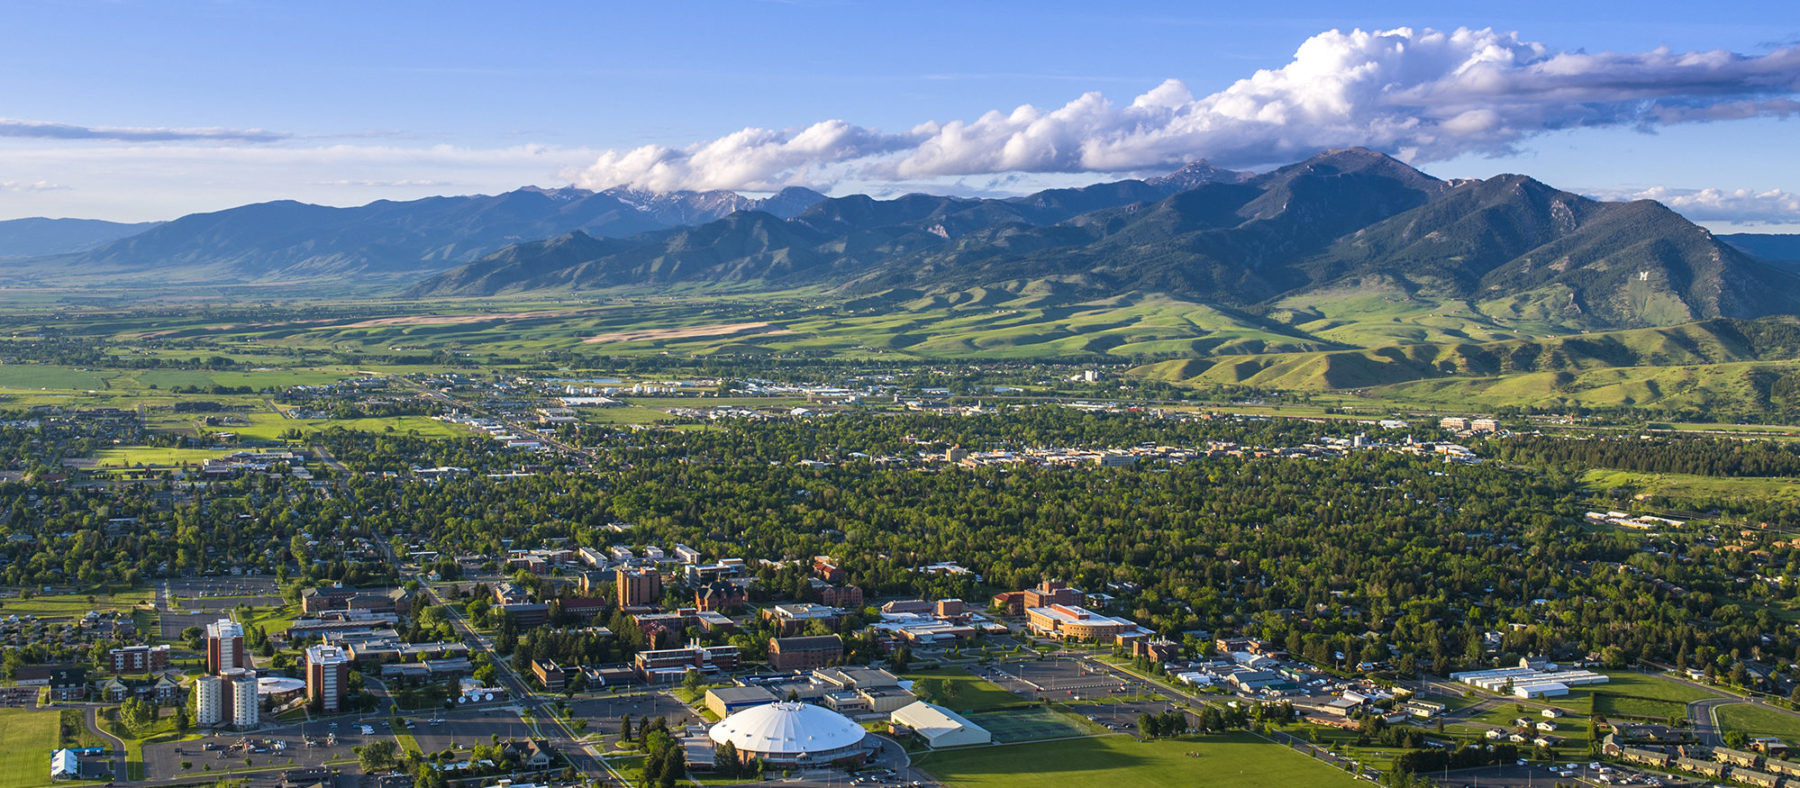
\includegraphics[width=5in,height=\textheight]{images/msu-campus.jpg}}
\usepackage{etoolbox}
\makeatletter
\providecommand{\subtitle}[1]{% add subtitle to \maketitle
  \apptocmd{\@title}{\par {\large #1 \par}}{}{}
}
\makeatother
\subtitle{Spring 2025\\
Montana State University}
\author{Melinda Yager\\
Jade Schmidt\\
Stacey Hancock}
\date{}

\begin{document}
\maketitle

\newpage
\thispagestyle{empty}

This resource was developed by Melinda Yager, Jade Schmidt, and Stacey Hancock in 2021 to accompany the online textbook: Hancock, S., Carnegie, N., Meyer, E., Schmidt, J., and Yager, M. (2021). \emph{Montana State Introductory Statistics with R}. Montana State University. \url{https://mtstateintrostats.github.io/IntroStatTextbook/}.

This resource is released under a \href{https://creativecommons.org/licenses/by-nc-sa/4.0/}{Creative Commons BY-NC-SA 4.0} license unless otherwise noted.

\setcounter{tocdepth}{1}
\addtocontents{toc}{\protect\thispagestyle{empty}}
\tableofcontents
\thispagestyle{empty}

\newpage
\setcounter{page}{1}

\chapter*{Preface}\label{preface}
\addcontentsline{toc}{chapter}{Preface}

This coursepack accompanies the textbook for STAT 216: Montana State Introductory Statistics with R, which can be found at \url{https://mtstateintrostats.github.io/IntroStatTextbook/}. The syllabus for the course (including the course calendar), data sets, and links to D2L Brightspace, Gradescope, and the MSU RStudio server can be found on the course webpage: \url{https://math.montana.edu/courses/s216/}.
Other notes and review materials are linked in D2L.

Each of the activities in this workbook is designed to target specific learning outcomes of the course, giving you practice with important statistical concepts in a group setting with instructor guidance. In addition to the in-class activities for the course, video notes are provided to aid in taking notes while you complete the required videos. Bring this workbook with you to class each class period, and take notes in the workbook as you would your own notes. A well-written completed workbook will provide an optimal study guide for exams!

All activities and labs in this coursepack will be completed during class time. Parts of each lab will be turned in on Gradescope. To aid in your understanding, read through the introduction for each activity before attending class each day.

STAT 216 is a 3-credit in-person course. In our experience, it takes six to nine hours per week outside of class to achieve a good grade in this class. By ``good'' we mean at least a C because a grade of D or below does not count toward fulfilling degree requirements. Many of you set your goals higher than just getting a C, and we fully support that. You need roughly nine hours per week to review past activities, read feedback on previous assignments, complete current assignments, and prepare for the next day's class. A typical week in the life of a STAT 216 student looks like:

\begin{itemize}
\tightlist
\item
  \emph{Prior to class meeting}:

  \begin{itemize}
  \tightlist
  \item
    Read assigned sections of the textbook, using the provided reading guides to take notes on the material.
  \item
    Watch the provided videos, taking notes in the coursepack.
  \item
    Read through the introduction to the day's in-class activity.
  \item
    Read through the week's homework assignment and note any questions you may have on the content.
  \end{itemize}
\item
  \emph{During class meeting}:

  \begin{itemize}
  \tightlist
  \item
    Work through the guided activity, in-class activity or weekly lab with your classmates and instructor, taking detailed notes on your answers to each question in the activity.
  \end{itemize}
\item
  \emph{After class meeting}:

  \begin{itemize}
  \tightlist
  \item
    Complete any parts of the activity you did not complete in class.
  \item
    Review the activity solutions in the Math and Stat Center, and take notes on key points.
  \item
    Complete any remaining assigned readings for the week.
  \item
    Complete the week's homework assignment.
  \end{itemize}
\end{itemize}

\nocite{*}

\chapter{Exploratory Data Analysis and Simulation-based Inference for Two Categorical Variables}\label{exploratory-data-analysis-and-simulation-based-inference-for-two-categorical-variables}

\section{Vocabulary Review and Key Topics}\label{vocabulary-review-and-key-topics}

Review the Golden Ticket posted in the resources at the end of the coursepack for a summary two categorical variables.

\subsection{Key topics}\label{key-topics}

Module 8 will introduce exploratory data analysis and simulation-based inference for two categorical variables. We also explore study design and confounding variables.

Types of plots for two categorical variables

\begin{itemize}
\item
  \textbf{Segmented bar plot}: plots the conditional proportion of the response outcomes in each explanatory variable group

  \begin{itemize}
  \tightlist
  \item
    The plot shows no association between the variables, if the height of each segment is approximately the same in each group
  \end{itemize}
\item
  \textbf{Mosaic plot}: similar to the segmented bar plot but the sample size is reflected by the width of the bars
\end{itemize}

Summary measures

\begin{itemize}
\item
  \textbf{Difference in proportion}: calculation of the difference in two conditional proportions

  \begin{itemize}
  \item
    Parameter notation: \(\pi_1 - \pi_2\)
  \item
    Sample notation: \(\hat{p}_1 - \hat{p}_2\)
  \end{itemize}
\item
  \textbf{Relative risk}: the ratio of the conditional proportions

  \begin{itemize}
  \tightlist
  \item
    \(\text{Relative Risk} = \frac{\hat{p}_1}{\hat{p}_2}\)
  \end{itemize}
\end{itemize}

Interpretation of relative risk:

\begin{itemize}
\item
  The risk of success in group 1 is relative risk times the risk of success in group 2
\item
  Can also interpret as a percent increase or percent decrease in risk
\end{itemize}

\[(RR-1) \times 100\%\]

\begin{verbatim}
* The risk of success in group 1 is xx\% higher or lower that the risk of success in group 2
\end{verbatim}

\begin{itemize}
\item
  Explanatory variable: the variable researchers think \emph{may be} affecting the other variable.
\item
  Response variable: the variable researchers think \emph{may be} influenced by the other variable.
\item
  Confounding variable:

  \begin{itemize}
  \tightlist
  \item
    associated with both the explanatory and the response variable
  \item
    explains the association shown by the data
  \end{itemize}
\end{itemize}

Study Design

\begin{itemize}
\item
  Observational study:
\item
  Randomized experiment:
\end{itemize}

Scope of Inference Table:

\begin{center}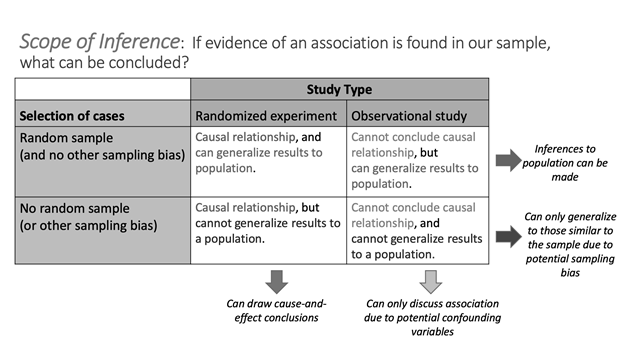
\includegraphics[width=0.65\linewidth]{images/ScopeOfInferenceGreyscale} \end{center}

\begin{itemize}
\item
  Conditions necessary to use simulation methods for inference for two categorical variables

  \begin{itemize}
  \tightlist
  \item
    There must be independence of observational units within groups and between groups
  \end{itemize}
\end{itemize}

\newpage

\section{Video Notes: Inference for Two Categorical Variables using Simulation-based Methods}\label{video-notes-inference-for-two-categorical-variables-using-simulation-based-methods}

Read Sections 2.2 - 2.4, 15.1, 15.2, Chapter 4 and Chapter 16 in the course textbook. Use the following videos to complete the video notes for Module 8.

\subsection{Course Videos}\label{course-videos}

\begin{itemize}
\item
  2.2to2.4
\item
  4.1\_TwoProp
\item
  4.2\_TwoProp
\item
  4.4
\item
  15.1
\item
  15.2
\item
  RelativeRisk
\end{itemize}

\subsection*{Observational studies, experiments, and scope of inference: Video 2.2to2.4}\label{observational-studies-experiments-and-scope-of-inference-video-2.2to2.4}
\addcontentsline{toc}{subsection}{Observational studies, experiments, and scope of inference: Video 2.2to2.4}

\begin{itemize}
\item
  Review

  \begin{itemize}
  \item
    Explanatory variable: the variable researchers think \emph{may be} affecting the other variable.
  \item
    Response variable: the variable researchers think \emph{may be} influenced by the other variable.
  \end{itemize}
\item
  Confounding variable:

  \begin{itemize}
  \tightlist
  \item
    associated with both the explanatory and the response variable
  \item
    explains the association shown by the data
  \end{itemize}
\end{itemize}

Example:

\vspace{0.8in}

\subsubsection*{Study design}\label{study-design}
\addcontentsline{toc}{subsubsection}{Study design}

\begin{itemize}
\tightlist
\item
  Observational study:
\end{itemize}

\vspace{0.5in}

\begin{itemize}
\tightlist
\item
  Experiment:
\end{itemize}

\vspace{0.5in}

Principles of experimental design

\begin{itemize}
\item
  Control: hold other differences constant across groups
  \vspace{1mm}
\item
  Randomization: randomized experiment
  \vspace{1mm}
\item
  Replication: large sample size or repeat of study
  \vspace{1mm}
\item
  Blocking: group based on certain characteristics
  \vspace{1mm}
\end{itemize}

Example: It is well known that humans have more difficulty differentiating between faces of people from different races than people within their own race. A 2018 study published in the Journal of Experimental Psychology (Levin 2000): Human Perception and Performance investigated a similar phenomenon with gender. In the study, volunteers were shown several pictures of strangers. Half the volunteers were randomly assigned to rate the attractiveness of the individuals pictured. The other half were told to rate the distinctiveness of the faces seen. Both groups were then shown a slideshow of faces (some that had been rated in the first part of the study, some that were new to the volunteer) and asked to determine if each face was old or new. Researchers found people were better able to recognize faces of their own gender when asked to rate the distinctiveness of the faces, compared to when asked to rate the attractiveness of the faces.

\begin{itemize}
\tightlist
\item
  What is the study design?
\end{itemize}

\vspace{0.5in}

Example: In the Physician's Health Study ({``Physician's Health Study,''} n.d.), male physicians participated in a study to determine whether taking a daily low-dose aspirin reduced the risk of heart attacks. The male physicians were randomly assigned to the treatment groups. After five years, 104 of the 11,037 male physicians taking a daily low-dose aspirin had experienced a heart attack while 189 of the 11,034 male physicians taking a placebo had experienced a heart attack.

\begin{itemize}
\tightlist
\item
  What is the study design?
\end{itemize}

\vspace{0.5in}

\begin{itemize}
\tightlist
\item
  Assuming these data provide evidence that the low-dose aspirin group had a lower rate of heart attacks than the placebo group, is it valid for the researchers to conclude the lower rate of heart attacks was caused by the daily low-dose aspirin regimen?
\end{itemize}

\vspace{0.5in}

\subsubsection*{Scope of Inference}\label{scope-of-inference}
\addcontentsline{toc}{subsubsection}{Scope of Inference}

\begin{enumerate}
\def\labelenumi{\arabic{enumi}.}
\tightlist
\item
  How was the sample selected?
\end{enumerate}

\begin{itemize}
\tightlist
\item
  Random sample with no sampling bias:
\end{itemize}

\vspace{0.35in}

\begin{itemize}
\tightlist
\item
  Non-random sample with sampling bias:
\end{itemize}

\vspace{0.35in}

\begin{enumerate}
\def\labelenumi{\arabic{enumi}.}
\setcounter{enumi}{1}
\tightlist
\item
  What is the study design?
\end{enumerate}

\begin{itemize}
\tightlist
\item
  Randomized experiment:
\end{itemize}

\vspace{0.35in}

\begin{itemize}
\tightlist
\item
  Observational study:
\end{itemize}

\vspace{0.35in}

\newpage

Scope of Inference Table:

\begin{center}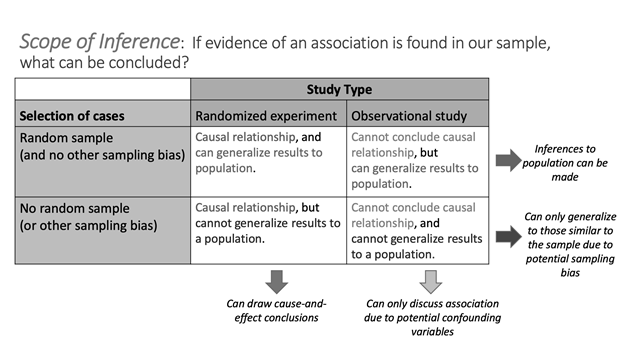
\includegraphics[width=0.65\linewidth]{images/ScopeOfInferenceGreyscale} \end{center}

Example: It is well known that humans have more difficulty differentiating between faces of people from different races than people within their own race. A 2018 study published in the Journal of Experimental Psychology (Levin 2000): Human Perception and Performance investigated a similar phenomenon with gender. In the study, volunteers were shown several pictures of strangers. Half the volunteers were randomly assigned to rate the attractiveness of the individuals pictured. The other half were told to rate the distinctiveness of the faces seen. Both groups were then shown a slideshow of faces (some that had been rated in the first part of the study, some that were new to the volunteer) and asked to determine if each face was old or new. Researchers found people were better able to recognize faces of their own gender when asked to rate the distinctiveness of the faces, compared to when asked to rate the attractiveness of the faces.

\begin{itemize}
\tightlist
\item
  What is the scope of inference for this study?
\end{itemize}

\vspace{0.5in}

\setstretch{1}

\newpage

\subsection*{Summarizing two categorical variables - Video 4.1\_TwoProp}\label{summarizing-two-categorical-variables---video-4.1_twoprop}
\addcontentsline{toc}{subsection}{Summarizing two categorical variables - Video 4.1\_TwoProp}

\begin{itemize}
\tightlist
\item
  The summary measure for two categorical variables is the \_\_\_\_\_\_\_\_\_\_\_\_\_\_\_\_\_\_\_\_\_\_ in \_\_\_\_\_\_\_\_\_\_\_\_\_\_\_\_\_\_\_\_\_\_\_\_\_\_\_\_\_.
\end{itemize}

Notation used for the population difference in proportion:

\begin{itemize}
\tightlist
\item
  Two categorical variables:
\end{itemize}

\vspace{0.2in}

\rgi \rgi - Subscripts represent the \_\_\_\_\_\_\_\_\_\_\_\_\_\_\_\_\_\_ variable groups

Notation used for the sample difference in proportion:

\begin{itemize}
\tightlist
\item
  Two categorical variables
\end{itemize}

\vspace{0.2in}

When we have two categorical variables we report the data in a \_\_\_\_\_\_\_\_\_\_\_\_\_\_\_ or two-way table with the \_\_\_\_\_\_\_\_\_\_\_\_\_\_\_ variable on the columns and the \_\_\_\_\_\_\_\_\_\_\_\_ variable on the rows.

\setstretch{1}

\vspace{2mm}

For today's videos we will again use the \texttt{moving\_to\_mt} data set.

Example from the Video: Gallatin Valley is the fastest growing county in Montana. You'll often hear Bozeman residents complaining about the `out-of-staters' moving in. A local real estate agent recorded data on a random sample of 100 home sales over the last year at her company and noted where the buyers were moving from as well as the age of the person or average age of a couple buying a home. The variable age was binned into two categories, ``Under30'' and ``Over30.'' Additionally, the variable, state the buyers were moving from, was created as a binary variable, ``Out'' for a location out of state and ``In'' for a location in state.

The following code reads in the data set, \texttt{moving\_to\_mt} and names the object moving.

\begin{Shaded}
\begin{Highlighting}[]
\NormalTok{moving }\OtherTok{\textless{}{-}} \FunctionTok{read.csv}\NormalTok{(}\StringTok{"data/moving\_to\_mt.csv"}\NormalTok{)}
\end{Highlighting}
\end{Shaded}

To look at the relationship between the variable, \texttt{Age\_Group} and the variable, \texttt{From} create the following two-way table using the \texttt{R} output below. Note, we are using \texttt{From} as the explanatory variable to predict whether a home sale has a buyer that is over or under the age of 30.

\begin{Shaded}
\begin{Highlighting}[]
\NormalTok{moving }\SpecialCharTok{\%\textgreater{}\%}
    \FunctionTok{group\_by}\NormalTok{(Age\_Group) }\SpecialCharTok{\%\textgreater{}\%} \FunctionTok{count}\NormalTok{(From) }\SpecialCharTok{\%\textgreater{}\%} \FunctionTok{print}\NormalTok{(}\AttributeTok{n=}\DecValTok{8}\NormalTok{)}
\end{Highlighting}
\end{Shaded}

\begin{verbatim}
#> # A tibble: 8 x 3
#> # Groups:   Age_Group [2]
#>   Age_Group From      n
#>   <chr>     <chr> <int>
#> 1 Over30    CA        6
#> 2 Over30    CO        2
#> 3 Over30    MT       47
#> 4 Over30    WA       10
#> 5 Under30   CA        6
#> 6 Under30   CO        6
#> 7 Under30   MT       14
#> 8 Under30   WA        9
\end{verbatim}

\begin{center}
\begingroup
\setlength{\tabcolsep}{14pt} % Default value: 6pt
\renewcommand{\arraystretch}{2} % Default value: 1
\begin{tabular}{|c|c|c|c|c|c|}
\hline
 & \multicolumn{4}{|c|}{\textbf{State}} & \\ \hline
\textbf{Age Group} & CA & CO & MT & WA & Total \\ \hline
 Over30 & 6 & 2 & 47 & 10 & 65 \\ \hline
 Under30 & 6 & 6 & 14 & 9 & 35 \\ \hline
 Total & 12 & 8 & 61 & 19 & 100\\ \hline
\end{tabular}
\endgroup
\end{center}

\begin{itemize}
\tightlist
\item
  Using the table above, how many of the sampled home sales have buyers who were under 30 years old and from Montana?
\end{itemize}

\vspace{0.2in}

\setstretch{1.5}

If we want to know what proportion of each age group is from each state, we would calculate the proportion of home sales with buyers from each state within each age group. In other words, divide the number of home sales from each state with buyers that are over 30 by the total for row 1, the total number of home sales with buyers over 30.

\setstretch{1}

\begin{itemize}
\tightlist
\item
  What proportion of sampled home sales with buyers under 30-years-old were from California?
\end{itemize}

\vspace{0.3in}

\begin{itemize}
\tightlist
\item
  What notation should be used for this value?
\end{itemize}

\vspace{0.2in}

\setstretch{1.5}

Additionally, we could find the proportion of home sales with buyers in each state for each age group. Here we would calculate the proportion of home sales with buyers in each age group within each state. Divide the number of home sales with buyers in each age group from CA by the total for column 1, the total number of home sales with buyers from CA.

\setstretch{1}

\begin{center}
\begingroup
\setlength{\tabcolsep}{14pt} % Default value: 6pt
\renewcommand{\arraystretch}{2} % Default value: 1
\begin{tabular}{|c|c|c|c|c|c|}
\hline
 & \multicolumn{4}{|c|}{\textbf{State}} & \\ \hline
\textbf{Age Group} & CA & CO & MT & WA & Total \\ \hline
 Over30 & 6 & 2 & 47 & 10 & 65 \\ \hline
 Under30 & 6 & 6 & 14 & 9 & 35 \\ \hline
 Total & 12 & 8 & 61 & 19 & 100\\ \hline
\end{tabular}
\endgroup
\end{center}

\begin{itemize}
\tightlist
\item
  Using the table, calculate the proportion of home sales in Gallatin County with in-state buyers who are over 30 years old? Use appropriate notation with informative subscripts.
\end{itemize}

\vspace{0.4in}

\begin{itemize}
\tightlist
\item
  Using the table, calculate the proportion of home sales in Gallatin County with California buyers who are over 30 years old? Use appropriate notation with informative subscripts.
\end{itemize}

\vspace{0.4in}

\begin{itemize}
\tightlist
\item
  Calculate the difference in proportion of home sales in Gallatin County over 30 years old from other parts of Montana and from California. Use MT - CA as the order of subtraction. Give appropriate notation.
\end{itemize}

\vspace{0.4in}

\begin{itemize}
\tightlist
\item
  Interpret the difference in proportion in context of the study.
\end{itemize}

\vspace{0.5in}

\subsection*{Plots for two categorical variables - Video 4.2\_TwoProp}\label{plots-for-two-categorical-variables---video-4.2_twoprop}
\addcontentsline{toc}{subsection}{Plots for two categorical variables - Video 4.2\_TwoProp}

In a segmented bar plot, the bar for each category will sum to 1. In this first plot, we are plotting the row proportions calculated conditional on the age group.

\begin{Shaded}
\begin{Highlighting}[]
\NormalTok{moving }\SpecialCharTok{\%\textgreater{}\%}
  \FunctionTok{ggplot}\NormalTok{(}\FunctionTok{aes}\NormalTok{(}\AttributeTok{x =}\NormalTok{ Age\_Group, }\AttributeTok{fill =}\NormalTok{ From))}\SpecialCharTok{+} \CommentTok{\#Enter the variables to plot}
  \FunctionTok{geom\_bar}\NormalTok{(}\AttributeTok{stat =} \StringTok{"count"}\NormalTok{, }\AttributeTok{position =} \StringTok{"fill"}\NormalTok{) }\SpecialCharTok{+}
  \FunctionTok{labs}\NormalTok{(}\AttributeTok{title =} \StringTok{"Segmented bar plot of Age Group of Buyers by State of}
\StringTok{       Origin for Gallatin County Home Sales"}\NormalTok{,}
       \CommentTok{\#Title your plot}
       \AttributeTok{y =} \StringTok{"Relative Frequency"}\NormalTok{, }\CommentTok{\#y{-}axis label}
       \AttributeTok{x =} \StringTok{"Age Group"}\NormalTok{) }\SpecialCharTok{+} \CommentTok{\#x{-}axis label}
  \FunctionTok{scale\_fill\_grey}\NormalTok{()}
\end{Highlighting}
\end{Shaded}

\begin{center}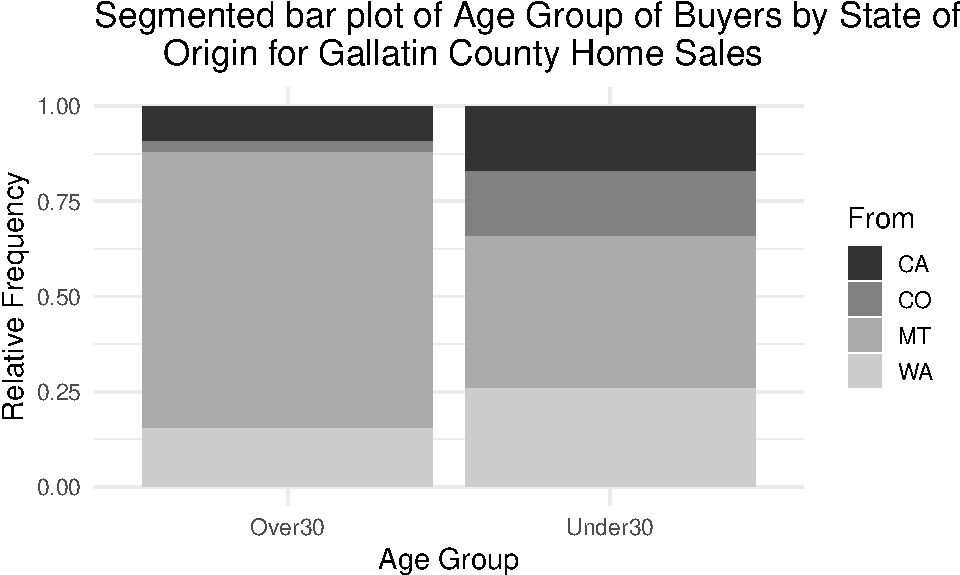
\includegraphics[width=0.55\linewidth]{08-VN08-two-cat-simulation_files/figure-latex/unnamed-chunk-4-1} \end{center}

In this second plot, we are plotting the column proportions calculated conditional on the state of origin for the buyer.

\begin{Shaded}
\begin{Highlighting}[]
\NormalTok{moving }\SpecialCharTok{\%\textgreater{}\%}
  \FunctionTok{ggplot}\NormalTok{(}\FunctionTok{aes}\NormalTok{(}\AttributeTok{x =}\NormalTok{ From , }\AttributeTok{fill =}\NormalTok{ Age\_Group))}\SpecialCharTok{+} \CommentTok{\#Enter variables to plot}
  \FunctionTok{geom\_bar}\NormalTok{(}\AttributeTok{stat =} \StringTok{"count"}\NormalTok{, }\AttributeTok{position =} \StringTok{"fill"}\NormalTok{) }\SpecialCharTok{+}
  \FunctionTok{labs}\NormalTok{(}\AttributeTok{title =} \StringTok{"Segmented bar plot of State of Origin of Buyers by Age}
\StringTok{       Group for Gallatin County Home Sales"}\NormalTok{,}
       \CommentTok{\#Title your plot}
       \AttributeTok{y =} \StringTok{"Relative Frequency"}\NormalTok{, }\CommentTok{\#y{-}axis label}
       \AttributeTok{x =} \StringTok{"State of Origin"}\NormalTok{) }\SpecialCharTok{+} \CommentTok{\#x{-}axis label}
  \FunctionTok{scale\_fill\_grey}\NormalTok{()}
\end{Highlighting}
\end{Shaded}

\begin{center}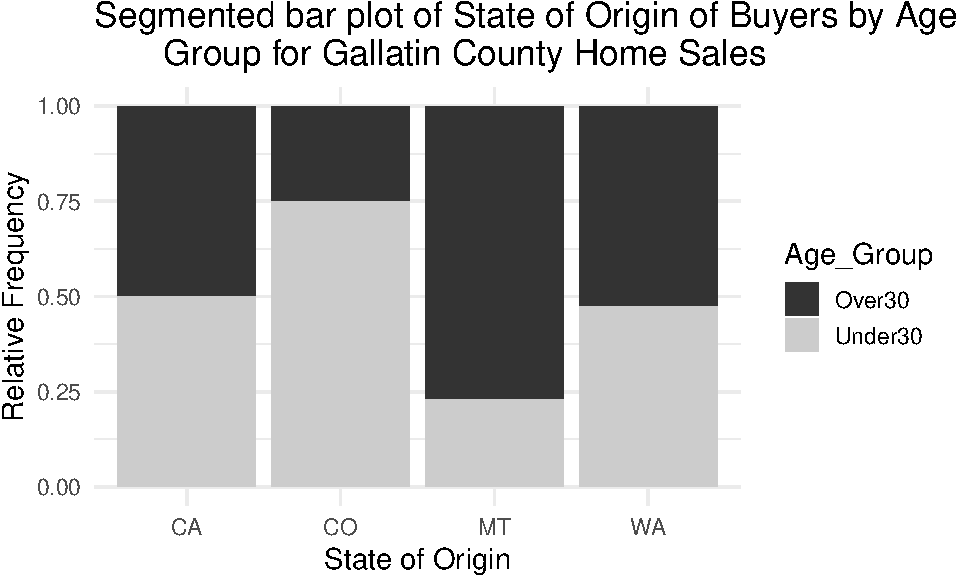
\includegraphics[width=0.55\linewidth]{08-VN08-two-cat-simulation_files/figure-latex/unnamed-chunk-5-1} \end{center}

Mosaic plot:

\begin{Shaded}
\begin{Highlighting}[]
\NormalTok{moving}\SpecialCharTok{$}\NormalTok{Age\_Group }\OtherTok{\textless{}{-}} \FunctionTok{factor}\NormalTok{(moving}\SpecialCharTok{$}\NormalTok{Age\_Group, }\AttributeTok{levels =} \FunctionTok{c}\NormalTok{(}\StringTok{"Under30"}\NormalTok{, }\StringTok{"Over30"}\NormalTok{))}
\NormalTok{moving }\SpecialCharTok{\%\textgreater{}\%} \CommentTok{\# Data set piped into...}
  \FunctionTok{ggplot}\NormalTok{() }\SpecialCharTok{+}   \CommentTok{\# This specifies the variables}
  \FunctionTok{geom\_mosaic}\NormalTok{(}\FunctionTok{aes}\NormalTok{(}\AttributeTok{x=}\FunctionTok{product}\NormalTok{(From), }\AttributeTok{fill =}\NormalTok{ Age\_Group)) }\SpecialCharTok{+}
    \CommentTok{\# Tell it to make a mosaic plot}
  \FunctionTok{labs}\NormalTok{(}\AttributeTok{title =} \StringTok{"Mosaic plot of State of Origin Segmented by}
\StringTok{  Age Group for Gallatin County Home Sales"}\NormalTok{,}
       \CommentTok{\# Title your plot}
       \AttributeTok{x =} \StringTok{"State of Origin"}\NormalTok{,   }\CommentTok{\# Label the x axis}
       \AttributeTok{y =} \StringTok{""}\NormalTok{) }\SpecialCharTok{+}  \CommentTok{\# Remove y axis label}
    \FunctionTok{scale\_fill\_grey}\NormalTok{(}\AttributeTok{guide =} \FunctionTok{guide\_legend}\NormalTok{(}\AttributeTok{reverse =} \ConstantTok{TRUE}\NormalTok{)) }\CommentTok{\# Make figure color}
\end{Highlighting}
\end{Shaded}

\begin{center}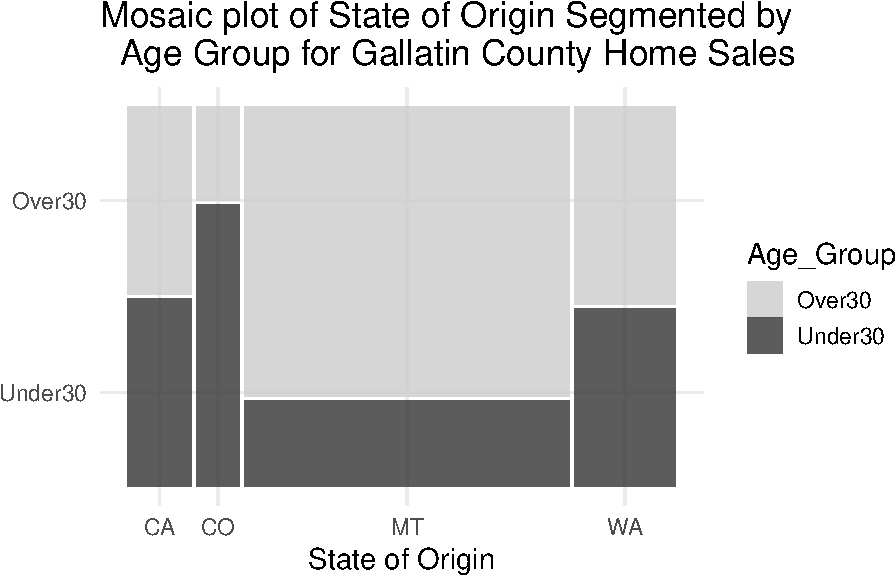
\includegraphics[width=0.75\linewidth]{08-VN08-two-cat-simulation_files/figure-latex/unnamed-chunk-6-1} \end{center}

\begin{itemize}
\tightlist
\item
  Why is the bar for MT the widest on the mosaic plot?
\end{itemize}

\vspace{0.2in}

\newpage

\subsubsection*{Simpson's paradox - Video 4.4}\label{simpsons-paradox---video-4.4}
\addcontentsline{toc}{subsubsection}{Simpson's paradox - Video 4.4}

\setstretch{1.5}

\begin{itemize}
\tightlist
\item
  When an apparent \_\_\_\_\_\_\_\_\_\_\_\_\_ between explanatory and response variables reverses when accounting for \_\_\_\_\_\_\_\_\_\_\_\_\_\_ variable.
\end{itemize}

\setstretch{1}

Example: The ``Berkeley Dataset'' contains all 12,763 applicants to UC-Berkeley's graduate programs in Fall 1973. This dataset was published by UC Berkeley researchers in an analysis to understand the possible gender bias in admissions and has now become a classic example of Simpson's Paradox.

\begin{Shaded}
\begin{Highlighting}[]
\NormalTok{discrim }\OtherTok{\textless{}{-}} \FunctionTok{read.csv}\NormalTok{ (}\StringTok{"data/berkeley.csv"}\NormalTok{)}

\NormalTok{discrim }\SpecialCharTok{\%\textgreater{}\%}
  \FunctionTok{ggplot}\NormalTok{(}\FunctionTok{aes}\NormalTok{(}\AttributeTok{x =}\NormalTok{Gender, }\AttributeTok{fill =}\NormalTok{ Admission))}\SpecialCharTok{+}
  \FunctionTok{geom\_bar}\NormalTok{(}\AttributeTok{stat =} \StringTok{"count"}\NormalTok{, }\AttributeTok{position =} \StringTok{"fill"}\NormalTok{) }\SpecialCharTok{+}
  \FunctionTok{labs}\NormalTok{(}\AttributeTok{title =} \StringTok{"Segmented bar plot of Sex of Berkley Applicants by}
\StringTok{       Admission Status"}\NormalTok{,}
       \AttributeTok{y =} \StringTok{"Relative Frequency"}\NormalTok{,}
       \AttributeTok{x =} \StringTok{"Sex"}\NormalTok{) }\SpecialCharTok{+}
  \FunctionTok{scale\_fill\_grey}\NormalTok{()}
\end{Highlighting}
\end{Shaded}

\begin{center}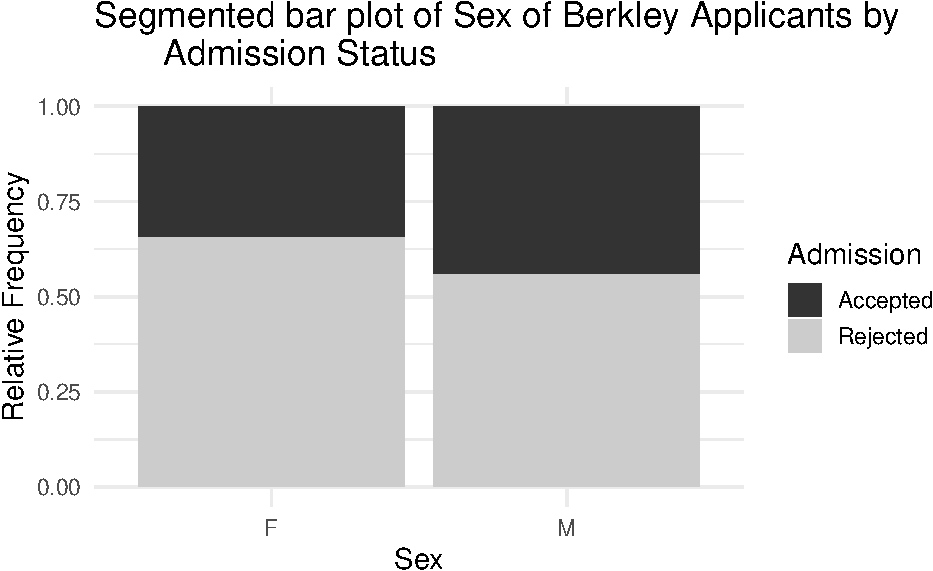
\includegraphics[width=0.85\linewidth]{08-VN08-two-cat-simulation_files/figure-latex/unnamed-chunk-7-1} \end{center}

The data showed that 44\% of male applicants were accepted and 35\% of female applicants were accepted. Does it appear that the female students are discriminated against?

\vspace{0.1in}

We can break down the data by major. A major code (either A, B, C, D, E, F, or Other) was used.

\newpage

Here we look at the relationship between admission status and sex for Program A and for Program B.

\begin{center}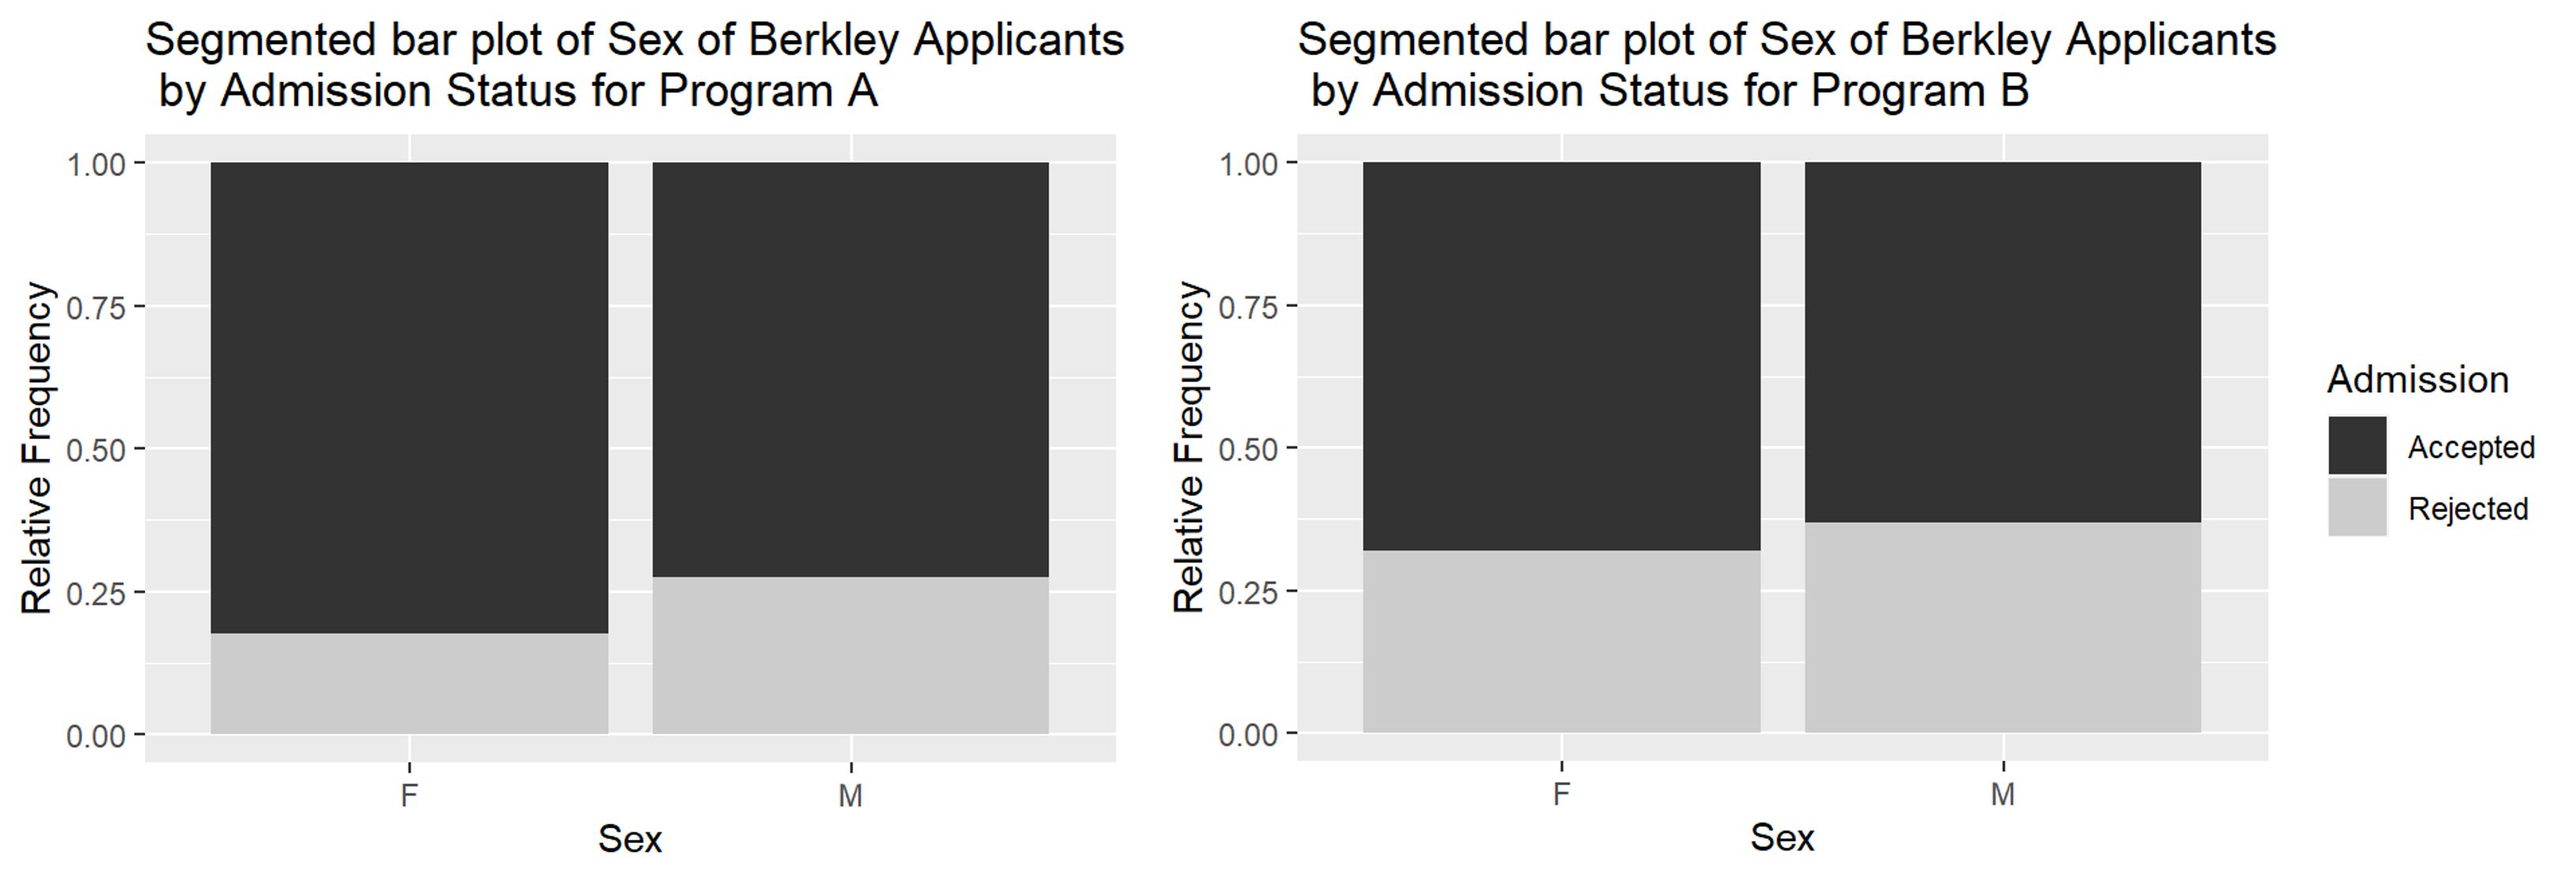
\includegraphics[width=0.85\linewidth]{images/SimPara_AB} \end{center}

Showing Program C and Program D.

\begin{center}\includegraphics[width=0.85\linewidth]{images/SimPara_cD} \end{center}

And finally, Program E and F.

\begin{center}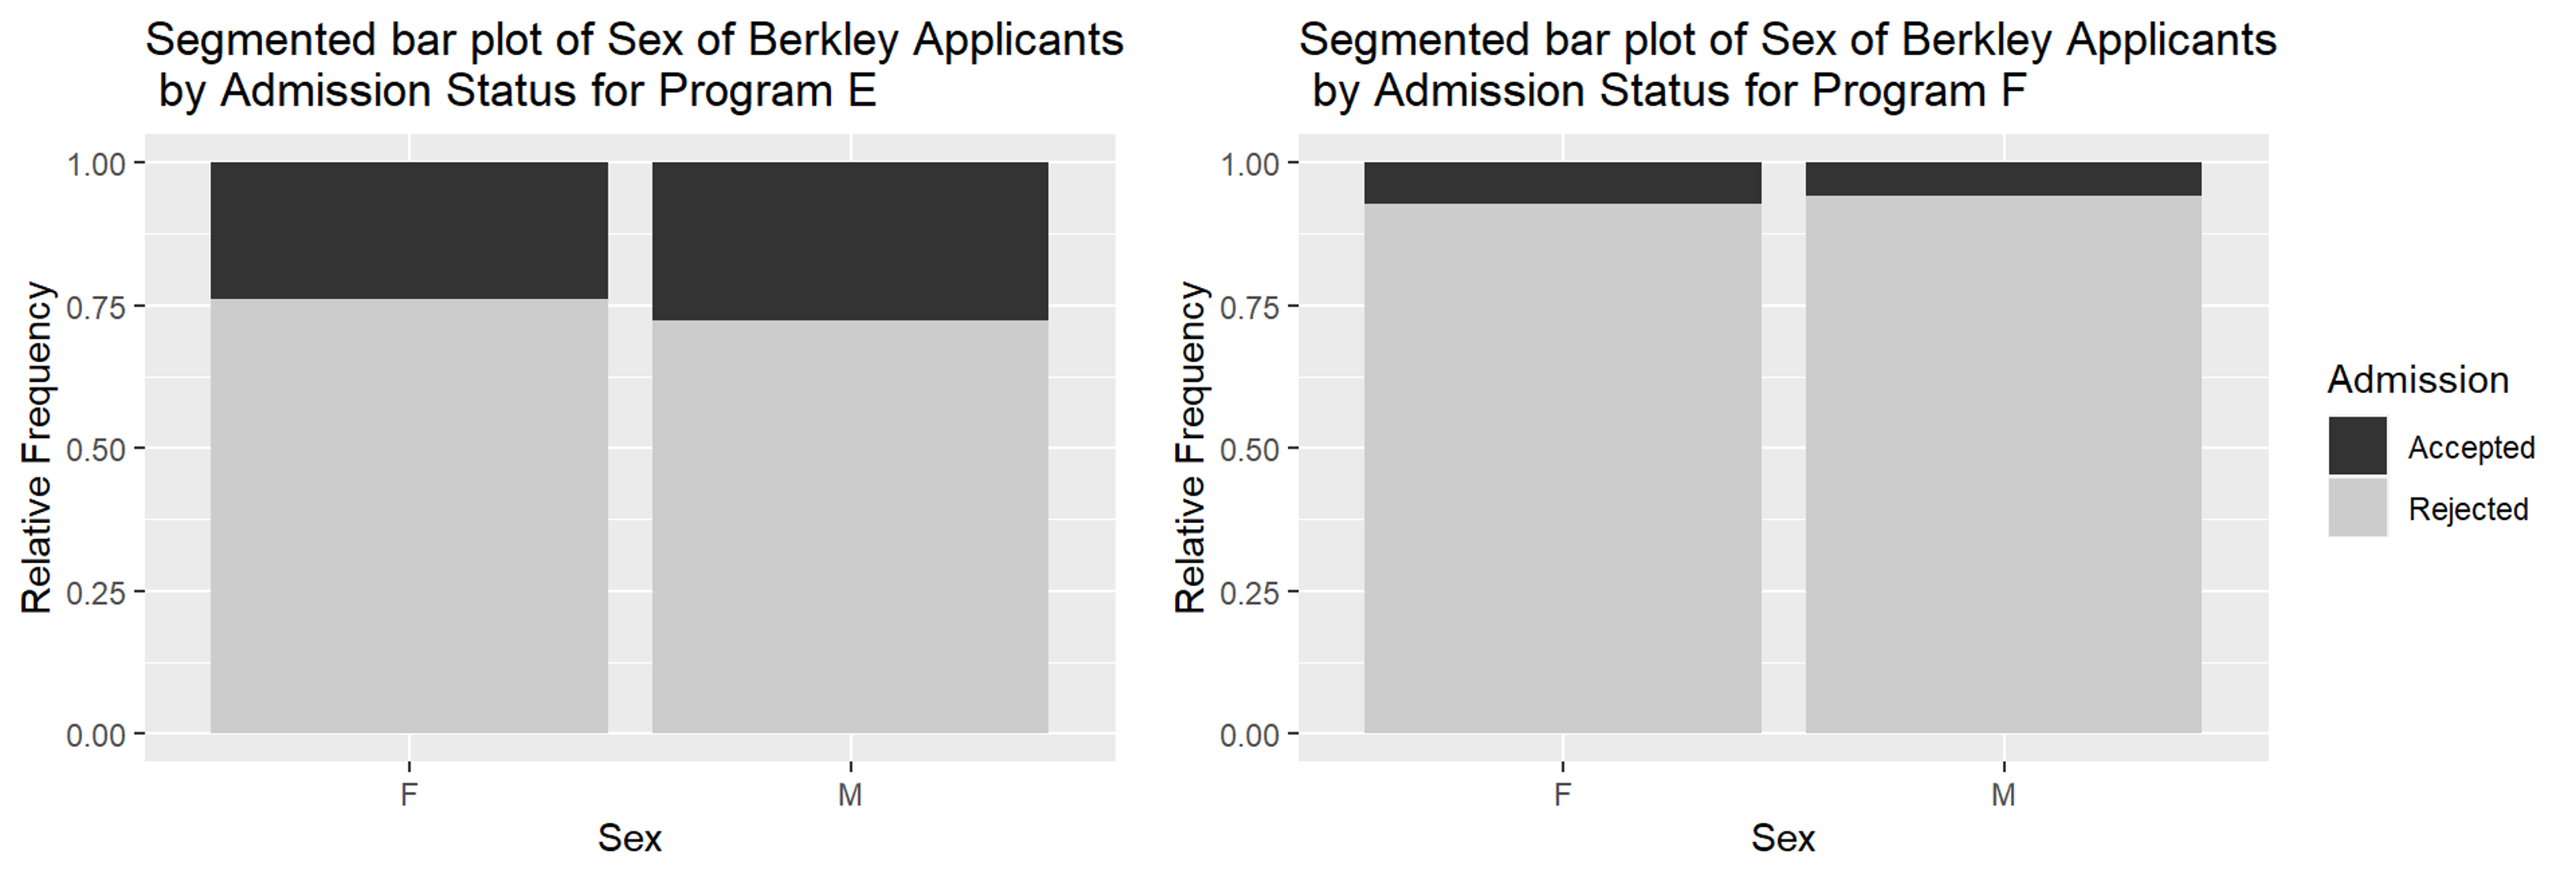
\includegraphics[width=0.85\linewidth]{images/SimPara_EF} \end{center}

We can see in several programs the acceptance rate is higher for females than for males.

\vspace{1in}

\newpage

\subsection*{Two categorical variables - Video 15.1}\label{two-categorical-variables---video-15.1}
\addcontentsline{toc}{subsection}{Two categorical variables - Video 15.1}

\setstretch{1.5}

\begin{itemize}
\tightlist
\item
  In this module, we will study inference for a \_\_\_\_\_\_\_\_\_\_\_\_\_\_\_\_\_\_\_\_\_\_ explanatory variable and a \_\_\_\_\_\_\_\_\_\_\_\_\_\_\_\_\_\_\_\_\_\_\_\_\_ response.
\end{itemize}

\setstretch{1}

Example: In a double-blind experiment (Weiss 1988) on 48 cocaine addicts hoping to overcome their addiction, half were randomly assigned to a drug called desipramine and the other half a placebo. The addicts were followed for 6 weeks to see whether they were still clean. Is desipramine more effective at helping cocaine addicts overcome their addiction than the placebo?

Observational units:

\vspace{0.15in}

Explanatory variable:

\vspace{0.15in}

Response variable:

\vspace{0.15in}

\setstretch{1.5}

Notation:

\begin{itemize}
\item
  Population proportion for group 1:
\item
  Population proportion for group 2:
\item
  Sample proportion for group 1:
\item
  Sample proportion for group 2:
\item
  Sample difference in proportions:
\item
  Sample size for group 1:
\item
  Sample size for group 2:
\end{itemize}

\setstretch{1}

\subsection*{Hypothesis Testing}\label{hypothesis-testing}
\addcontentsline{toc}{subsection}{Hypothesis Testing}

Conditions:

\begin{itemize}
\tightlist
\item
  Independence: the response for one observational unit will not influence another observational unit
\end{itemize}

Null hypothesis assumes ``no effect'', ``no difference'', ``nothing interesting happening'', etc.

\rgi Always of form: ``parameter'' = null value

\(H_0:\)

\vspace{0.2in}

\(H_A:\)

\vspace{0.2in}

\begin{itemize}
\tightlist
\item
  Research question determines the direction of the alternative hypothesis.
\end{itemize}

\newpage

Write the null and alternative hypotheses for the cocaine study:

In notation:

\(H_0:\)

\vspace{0.2in}

\(H_A:\)

\vspace{0.2in}

\subsubsection*{Summary statistics and plot}\label{summary-statistics-and-plot}
\addcontentsline{toc}{subsubsection}{Summary statistics and plot}

\begin{Shaded}
\begin{Highlighting}[]
\NormalTok{cocaine }\SpecialCharTok{\%\textgreater{}\%} \FunctionTok{group\_by}\NormalTok{(drug) }\SpecialCharTok{\%\textgreater{}\%} \FunctionTok{count}\NormalTok{(outcome)}
\end{Highlighting}
\end{Shaded}

\begin{verbatim}
#> # A tibble: 4 x 3
#> # Groups:   drug [2]
#>   drug        outcome      n
#>   <chr>       <chr>    <int>
#> 1 desipramine clean       14
#> 2 desipramine relapsed    10
#> 3 placebo     clean        4
#> 4 placebo     relapsed    20
\end{verbatim}

Summary statistic:

\vspace{0.3in}

Interpretation:

\vspace{0.4in}

\begin{Shaded}
\begin{Highlighting}[]
\NormalTok{cocaine}\SpecialCharTok{\%\textgreater{}\%}
  \FunctionTok{ggplot}\NormalTok{(}\FunctionTok{aes}\NormalTok{(}\AttributeTok{x =}\NormalTok{ drug, }\AttributeTok{fill =}\NormalTok{ outcome))}\SpecialCharTok{+}
  \FunctionTok{geom\_bar}\NormalTok{(}\AttributeTok{stat =} \StringTok{"count"}\NormalTok{, }\AttributeTok{position =} \StringTok{"fill"}\NormalTok{) }\SpecialCharTok{+}
  \FunctionTok{labs}\NormalTok{(}\AttributeTok{title =} \StringTok{"Bar plot of Type of Drug, Segmented by }
\StringTok{       Outcome for Cocaine Addicts"}\NormalTok{,}
       \AttributeTok{y =} \StringTok{"Relative Frequency"}\NormalTok{,}
       \AttributeTok{x =} \StringTok{"Drug or Placebo"}\NormalTok{) }\SpecialCharTok{+}
    \FunctionTok{scale\_fill\_grey}\NormalTok{()}
\end{Highlighting}
\end{Shaded}

\begin{center}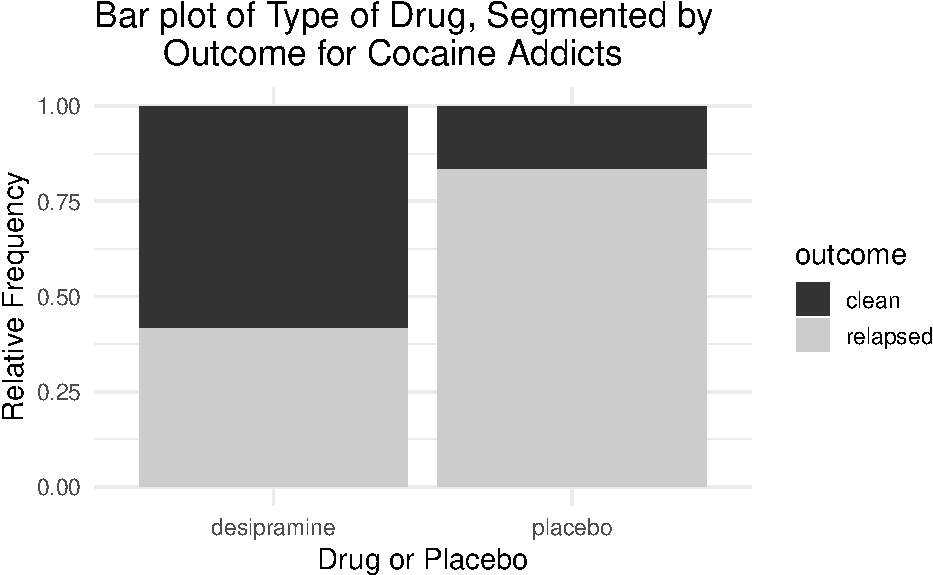
\includegraphics[width=0.6\linewidth]{08-VN08-two-cat-simulation_files/figure-latex/unnamed-chunk-13-1} \end{center}

Is the independence condition met for simulation inference?

\vspace{0.4in}

\subsubsection*{Simulation-based method}\label{simulation-based-method}
\addcontentsline{toc}{subsubsection}{Simulation-based method}

\begin{itemize}
\item
  Simulate many samples assuming \(H_0: \pi_1 = \pi_2\)

  \begin{itemize}
  \item
    Write the response variable values on cards
  \item
    Mix the explanatory variable groups together
  \item
    Shuffle cards into two explanatory variable groups to represent the sample size in each group (\(n_1\) and \(n_2\))
  \item
    Calculate and plot the simulated difference in sample proportions from each simulation
  \item
    Repeat 1000 times (simulations) to create the null distribution
  \item
    Find the proportion of simulations at least as extreme as \(\hat{p}_1 - \hat{p}_2\)
  \end{itemize}
\end{itemize}

\begin{Shaded}
\begin{Highlighting}[]
\FunctionTok{set.seed}\NormalTok{(}\DecValTok{216}\NormalTok{)}
\FunctionTok{two\_proportion\_test}\NormalTok{(}\AttributeTok{formula =}\NormalTok{ outcome}\SpecialCharTok{\textasciitilde{}}\NormalTok{drug, }\CommentTok{\# response \textasciitilde{} explanatory}
    \AttributeTok{data =}\NormalTok{ cocaine, }\CommentTok{\# Name of data set}
    \AttributeTok{first\_in\_subtraction =} \StringTok{"desipramine"}\NormalTok{, }\CommentTok{\# Order of subtraction: enter the name of Group 1}
    \AttributeTok{number\_repetitions =} \DecValTok{10000}\NormalTok{, }\CommentTok{\# Always use a minimum of 1000 repetitions}
    \AttributeTok{response\_value\_numerator =} \StringTok{"clean"}\NormalTok{, }\CommentTok{\# Define which outcome is a success}
    \AttributeTok{as\_extreme\_as =} \FloatTok{0.417}\NormalTok{, }\CommentTok{\# Calculated observed statistic (difference in sample proportions)}
    \AttributeTok{direction=}\StringTok{"greater"}\NormalTok{) }\CommentTok{\# Alternative hypothesis direction ("greater","less","two{-}sided")}
\end{Highlighting}
\end{Shaded}

\begin{center}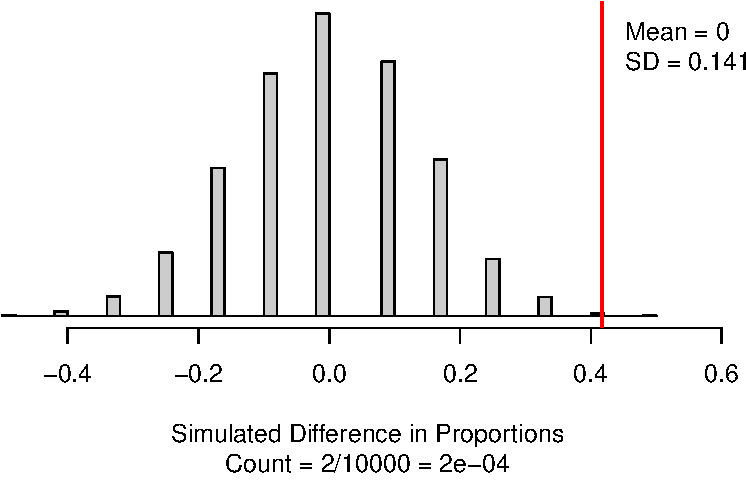
\includegraphics[width=0.7\linewidth]{08-VN08-two-cat-simulation_files/figure-latex/unnamed-chunk-14-1} \end{center}

Explain why the null distribution is centered at the value of zero:

\vspace{1in}

\newpage

Interpretation of the p-value:

\begin{itemize}
\item
  Statement about probability or proportion of samples
\item
  Statistic (summary measure and value)
\item
  Direction of the alternative
\item
  Null hypothesis (in context)
\end{itemize}

\vspace{0.8in}

Conclusion with scope of inference:

\begin{itemize}
\item
  Amount of evidence
\item
  Parameter of interest
\item
  Direction of the alternative hypothesis
\item
  Generalization
\item
  Causation
\end{itemize}

\vspace{0.8in}

\newpage

\subsection*{Confidence interval - Video 15.2}\label{confidence-interval---video-15.2}
\addcontentsline{toc}{subsection}{Confidence interval - Video 15.2}

To estimate the difference in true proportion we will create a confidence interval.

\subsubsection*{Simulation-based method}\label{simulation-based-method-1}
\addcontentsline{toc}{subsubsection}{Simulation-based method}

\begin{itemize}
\item
  Write the response variable values on cards
\item
  Keep explanatory variable groups separate
\item
  Sample with replacement \(n_1\) times in explanatory variable group 1 and \(n_2\) times in explanatory variable group 2
\item
  Calculate and plot the simulated difference in sample proportions from each simulation
\item
  Repeat 1000 times (simulations) to create the bootstrap distribution
\item
  Find the cut-offs for the middle X\% (confidence level) in a bootstrap distribution.
\end{itemize}

Returning to the cocaine example, we will estimate the difference in true proportion of cocaine addicts that stay clean for those on the desipramine and those on the placebo.

\begin{Shaded}
\begin{Highlighting}[]
\FunctionTok{set.seed}\NormalTok{(}\DecValTok{216}\NormalTok{)}
\FunctionTok{two\_proportion\_bootstrap\_CI}\NormalTok{(}\AttributeTok{formula =}\NormalTok{ outcome }\SpecialCharTok{\textasciitilde{}}\NormalTok{ drug, }
        \AttributeTok{data=}\NormalTok{cocaine, }\CommentTok{\# Name of data set}
        \AttributeTok{first\_in\_subtraction =} \StringTok{"desipramine"}\NormalTok{, }\CommentTok{\# Order of subtraction: enter the name of Group 1}
        \AttributeTok{response\_value\_numerator =} \StringTok{"clean"}\NormalTok{, }\CommentTok{\# Define which outcome is a success }
        \AttributeTok{number\_repetitions =} \DecValTok{10000}\NormalTok{, }\CommentTok{\# Always use a minimum of 1000 repetitions}
        \AttributeTok{confidence\_level =} \FloatTok{0.99}\NormalTok{) }\CommentTok{\# Enter the level of confidence as a decimal}
\end{Highlighting}
\end{Shaded}

\begin{center}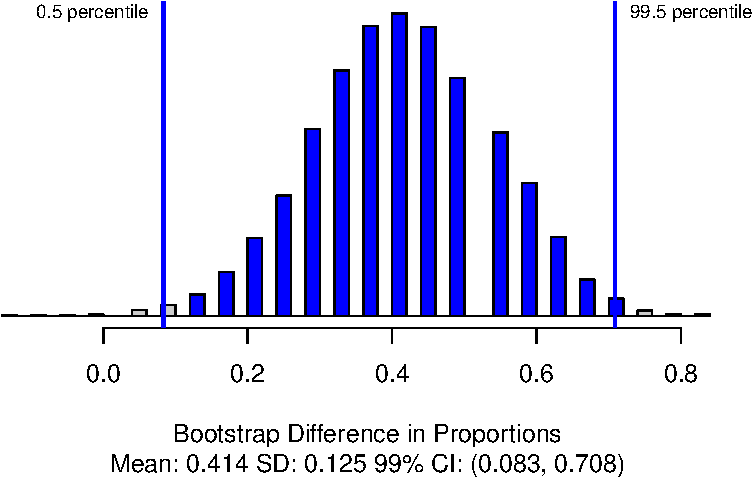
\includegraphics[width=0.7\linewidth]{08-VN08-two-cat-simulation_files/figure-latex/unnamed-chunk-15-1} \end{center}

Confidence interval interpretation:

\begin{itemize}
\item
  How confident you are (e.g., 90\%, 95\%, 98\%, 99\%)
\item
  Parameter of interest
\item
  Calculated interval
\item
  Order of subtraction when comparing two groups
\end{itemize}

\vspace{0.8in}

\subsection*{Relative Risk - Video RelativeRisk}\label{relative-risk---video-relativerisk}
\addcontentsline{toc}{subsection}{Relative Risk - Video RelativeRisk}

\begin{itemize}
\tightlist
\item
  Relative risk is the ratio of the risks in two different categories of an explanatory variable.
\end{itemize}

Relative Risk:

\vspace{0.3in}

Example: In a study reported in the New England Journal of Medicine (Du Toit 2015), one-hundred fifty (150) children who had shown sensitivity to peanuts were randomized to receive a flour containing a peanut protein or a placebo flour for 2.5 years. At age 5 years, children were tested with a standard skin prick to see if they had an allergic reaction to peanut protein (yes or no). 71\% of those in the peanut flour group no longer demonstrated a peanut allergy compared to 2\% of those in the placebo group.

\begin{itemize}
\tightlist
\item
  Calculate the relative risk of desensitization comparing the peanut flour group to the placebo group.
\end{itemize}

\vspace{0.8in}

\setstretch{1.5}

\begin{itemize}
\item
  Interpretation:

  \begin{itemize}
  \tightlist
  \item
    The proportion of successes in group 1 is the \(RR\) \_\_\_\_\_\_\_\_\_\_\_\_\_\_\_\_ the proportion of successes in group 2.
  \end{itemize}
\end{itemize}

Increase in risk:

\vspace{0.3in}

\begin{itemize}
\item
  Interpretation:

  \begin{itemize}
  \tightlist
  \item
    The proportion of successes in group 1 is the \((RR-1)\) \_\_\_\_\_\_\_\_\_\_\_\_\_\_
    higher/lower than the proportion of successes in group 2.
  \end{itemize}
\end{itemize}

Percent increase in risk:

\vspace{0.3in}

\begin{itemize}
\item
  Interpretation:

  \begin{itemize}
  \tightlist
  \item
    The proportion of successes in group 1 is the \((RR-1)\times 100\) \_\_\_\_\_\_\_\_\_\_ higher/lower than the proportion of successes in group 2.
  \end{itemize}
\end{itemize}

\setstretch{1}

\begin{itemize}
\tightlist
\item
  Interpret the value of relative risk from the peanut study in context of the problem.
\end{itemize}

\vspace{0.6in}

\begin{itemize}
\tightlist
\item
  Find the increase (or decrease) in risk of desensitization and interpret this value in context of the problem.
\end{itemize}

\vspace{1in}

\begin{itemize}
\tightlist
\item
  Find the percent increase (or decrease) in risk of desensitization and interpret this value in context of the problem.
\end{itemize}

\vspace{1in}

Within the peanut flour group, the percent desensitized within each age group (at start of study) is as follows:

1-year-olds: 71\%; 2-year-olds: 35\%; 3-year-olds: 19\%

\begin{itemize}
\tightlist
\item
  Calculate the relative risk of desensitization comparing the 3 year olds to the 2 year olds within the peanut flour group.
\end{itemize}

\vspace{0.8in}

\begin{itemize}
\tightlist
\item
  Interpret the percent increase (or decrease) in risk of desensitization comparing the 3 year olds to the 2 year olds within the peanut flour group.
\end{itemize}

\vspace{0.8in}

\subsubsection*{Relative risk in the news}\label{relative-risk-in-the-news}
\addcontentsline{toc}{subsubsection}{Relative risk in the news}

People 50 and older who have had a mild case of covid-19 are 15\% more likely to develop shingles (herpes zoster) within six months than are those who have not been infected by the coronavirus, according to research published in the journal Open Forum Infectious Diseases (Bhavsar 2022).

\begin{itemize}
\tightlist
\item
  What was the calculated relative risk of developing shingles when comparing those who has mild COVID-19 to those who had not had COVID-19, among the 50 and older population?
\end{itemize}

\vspace{0.8in}

\subsubsection*{Testing Relative Risk}\label{testing-relative-risk}
\addcontentsline{toc}{subsubsection}{Testing Relative Risk}

In Unit 2, we tested for a difference in proportion. We could also test for relative risk.

\setstretch{1.5}

Null Hypothesis:

\(H_0:\)

\vspace{0.2in}

Alternative Hypothesis:

\(H_A:\)

\vspace{0.2in}

\setstretch{1}

\subsection{Concept Check}\label{concept-check}

Be prepared for group discussion in the next class. One member from the table should write the answers to the following on the whiteboard.

\begin{enumerate}
\def\labelenumi{\arabic{enumi}.}
\tightlist
\item
  Explain why the null distribution is centered at the value of zero.
\end{enumerate}

\vspace{0.5in}

\begin{enumerate}
\def\labelenumi{\arabic{enumi}.}
\setcounter{enumi}{1}
\tightlist
\item
  Does the confidence interval agree with the p-value?
\end{enumerate}

\vspace{0.5in}

\begin{enumerate}
\def\labelenumi{\arabic{enumi}.}
\setcounter{enumi}{2}
\tightlist
\item
  What is the difference between a mosaic plot and a segmented bar plot?
\end{enumerate}

\vspace{0.5in}

\begin{enumerate}
\def\labelenumi{\arabic{enumi}.}
\setcounter{enumi}{3}
\tightlist
\item
  What does relative risk measure?
  \newpage
\end{enumerate}

\section{Activity 16: Study Design}\label{activity-16-study-design}

\setstretch{1}

\subsection{Learning outcomes}\label{learning-outcomes}

\begin{itemize}
\item
  Explain the purpose of random assignment and its effect on scope of inference.
\item
  Identify whether a study design is observational or an experiment.
\item
  Identify confounding variables in observational studies and explain why they are confounding.
\end{itemize}

\subsection{Terminology review}\label{terminology-review}

In this activity, we will examine different study designs, confounding variables, and how to determine the scope of inference for a study. Some terms covered in this activity are:

\begin{itemize}
\item
  Scope of inference
\item
  Explanatory variable
\item
  Response variable
\item
  Confounding variable
\item
  Experiment
\item
  Observational study
\end{itemize}

To review these concepts, see Sections 2.2 through 2.5 in the textbook.

\subsection{Atrial fibrillation}\label{atrial-fibrillation}

Atrial fibrillation is an irregular and often elevated heart rate. In some people, atrial fibrillation will come and go on its own, but others will experience this condition on a permanent basis. When atrial fibrillation is constant, medications are required to stabilize the patient's heart rate and to help prevent blood clots from forming. Pharmaceutical scientists at a large pharmaceutical company believe they have developed a new medication that effectively stabilizes heart rates in people with permanent atrial fibrillation. They set out to conduct a trial study to investigate the new drug. The scientists will need to compare the proportion of patients whose heart rate is stabilized between two groups of subjects, one of whom is given a placebo and the other given the new medication.

\begin{enumerate}
\def\labelenumi{\arabic{enumi}.}
\item
  Identify the explanatory and response variable in this trial study.

  Explanatory variable:
  \vspace{0.5in}

  Response variable:
  \vspace{0.5in}
\end{enumerate}

\newpage

Suppose 24 subjects with permanent atrial fibrillation have volunteered to participate in this study. There are 16 subjects that self-identified as male and 8 subjects that self-identified as female.

\begin{enumerate}
\def\labelenumi{\arabic{enumi}.}
\setcounter{enumi}{1}
\item
  One way to separate into two groups would be to give all the males the placebo and all the females the new drug. Explain why this is not a reasonable strategy.
  \vspace{1in}
\item
  Could the scientists fix the problem with the strategy presented in question 2 by creating equal sized groups by putting 4 males and 8 females into the drug group and the remaining 12 males in the placebo group? Explain your answer.
  \vspace{0.5in}
\item
  A third strategy would be to \textbf{block} on sex. In this type of study, the scientists would assign 4 females and 8 males to each group. Using this strategy, out of the 12 individuals in each group what \textbf{proportion} are males?
  \vspace{0.3in}
\item
  Assume the scientists used the strategy in question 4, but they put the four tallest females and eight tallest males into the drug group and the remaining subjects into the placebo group. They found that the proportion of patients whose heart rate stabilized is higher in the drug group than the placebo group.\\
  \vspace{0.1in}

  Could that difference be due to the sex of the subjects? Explain your answer.
  \vspace{0.5in}

  Could it be due to other variables? Explain your answer.
  \vspace{0.5in}
\end{enumerate}

While the strategy presented in question 5 controlled for the sex of the subject, there are more potential \textbf{confounding variables} in the study. A confounding variable is a variable that is \emph{both}

\begin{enumerate}
\def\labelenumi{\arabic{enumi}.}
\tightlist
\item
  associated with the explanatory variable, \emph{and}
\item
  associated with the response variable.
\end{enumerate}

When both these conditions are met, if we observe an association between the explanatory variable and the response variable in the data, we cannot be sure if this association is due to the explanatory variable or the confounding variable---the explanatory and confounding variables are ``confounded.''

\textbf{Random assignment} means that subjects in a study have an equally likely chance of receiving any of the available treatments.

\newpage

\begin{enumerate}
\def\labelenumi{\arabic{enumi}.}
\setcounter{enumi}{5}
\tightlist
\item
  You will now investigate how randomly assigning subjects impacts a study's scope of inference.
\end{enumerate}

\begin{itemize}
\item
  Navigate to the ``Randomizing Subjects'' applet under the ``Other Applets'' heading at: \url{http://www.rossmanchance.com/ISIapplets.html}. This applet lists the sex and height of each of the 24 subjects. Click ``Show Graphs'' to see a bar chart showing the sex of each subject. Currently, the applet is showing the strategy outlined in question 3.
\item
  Click ``Randomize''.
\end{itemize}

~~~In this random assignment, what proportion of males are in group 1 (the placebo group)?

\vspace{0.1in}

~~~What proportion of males are in group 2 (the drug group)?

\vspace{0.1in}

~~~What is the difference in proportion of males between the two groups (placebo - drug)?

\vspace{0.1in}

\begin{enumerate}
\def\labelenumi{\arabic{enumi}.}
\setcounter{enumi}{6}
\item
  Notice the difference in the two proportions is shown as a dot in the plot at the bottom of the web page. Un-check the box for Animate above ``Randomize'' and click ``Randomize'' again. Did you get the same difference in proportion of males between the placebo and drug groups?
  \vspace{0.25in}
\item
  Change ``Replications'' to 998 (for 1000 total). Click ``Randomize'' again. Sketch the plot of the distribution of difference in proportions from each of the 1000 random assignments here. Be sure to include a descriptive \(x\)-axis label.
  \vspace{1.25in}
\item
  Does random assignment \emph{always} balance the placebo and drug groups based on the sex of the participants? Does random assignment \emph{tend} to make the placebo and drug groups \emph{roughly} the same with respect to the distribution of sex? Use your plot from question 8 to justify your answers.
  \vspace{0.5in}
\item
  Change the drop-down menu below Group 2 from ``sex'' to ``height''. The applet now calculates the average height in the placebo and drug groups for each of the 1000 random assignments. The dot plot displays the distribution of the difference in mean heights (placebo - drug) for each random assignment. Based on this dot plot, is height distributed equally, on average, between the two groups? Explain how you know.
  \vspace{0.5in}
\end{enumerate}

\newpage

The diagram below summarizes these ideas about confounding variables and random assignment. When a confounding variable is present (such as sex or height), and an association is found in a study, it is impossible to discern what caused the change in the response variable. Is the change the result of the explanatory variable or the confounding variable? However, if all confounding variables are \emph{balanced} across the treatment groups, then only the explanatory variable differs between the groups and thus \emph{must have caused} the change seen in the response variable.

\begin{figure}

{\centering 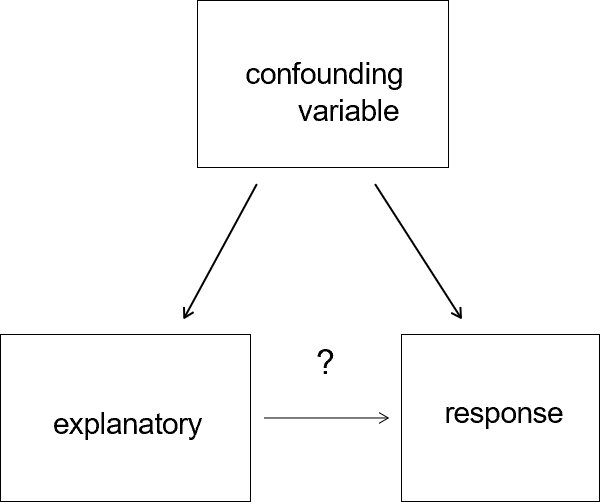
\includegraphics[width=0.4\linewidth]{images/confounding} 

}

\end{figure}

\begin{enumerate}
\def\labelenumi{\arabic{enumi}.}
\setcounter{enumi}{10}
\item
  What is the purpose of random assignment of the subjects in a study to the explanatory variable groups? Cross out the arrow in the figure above that is eliminated by random assignment.
  \vspace{0.8in}
\item
  Suppose in this study on atrial fibrillation, the scientists did randomly assign groups and found that the drug group has a higher proportion of subjects whose heart rates stabilized than the placebo group. Can the scientists conclude the new drug \emph{caused} the increased chance of stabilization? Explain your answer.
  \vspace{0.8in}
\item
  Is the sample of subjects a simple random sample or a convenience sample?
\end{enumerate}

\vspace{0.3in}

\begin{enumerate}
\def\labelenumi{\arabic{enumi}.}
\setcounter{enumi}{13}
\tightlist
\item
  Both the sampling method and the study design will help to determine the \emph{scope of inference} for a study: To \emph{whom} can we generalize, and can we conclude \emph{causation or only association}? Use your answers to question 12 and 13 and the table on the next page to determine the scope of inference of this trial study described in question 12.
  \vspace{0.3in}
\end{enumerate}

\begin{center}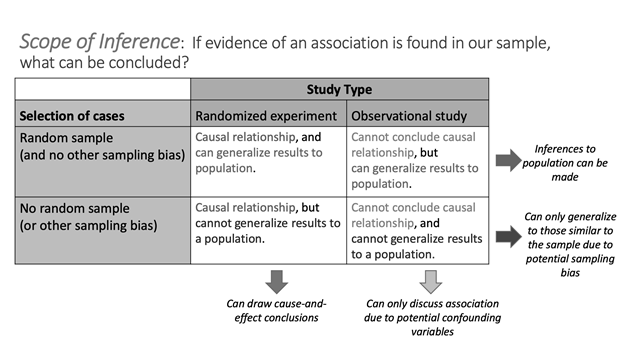
\includegraphics[width=0.75\linewidth]{images/ScopeOfInferenceGreyscale} \end{center}

\subsection{Scope of Inference}\label{scope-of-inference-1}

The two main study designs we will cover are \textbf{observational studies} and \textbf{experiments}. In observational studies, researchers have no influence over which subjects are in each group being compared (though they can control other variables in the study). An experiment is defined by assignment of the treatment groups of the \emph{explanatory variable}, typically via random assignment.

For the next exercises identify the study design (observational study or experiment), the sampling method, and the scope of inference.

\begin{enumerate}
\def\labelenumi{\arabic{enumi}.}
\setcounter{enumi}{14}
\item
  The pharmaceutical company Moderna Therapeutics, working in conjunction with the National Institutes of Health, conducted Phase 3 clinical trials of a vaccine for COVID-19 in the Fall of 2021. US clinical research sites enrolled 30,000 volunteers without COVID-19 to participate. Participants were randomly assigned to receive either the candidate vaccine or a saline placebo. They were then followed to assess whether or not they developed COVID-19. The trial was double-blind, so neither the investigators nor the participants knew who was assigned to which group.
  \vspace{0.1in}

  Study design:
  \vspace{0.3in}

  Sampling method:
  \vspace{0.3in}

  Scope of inference:
  \newpage
\item
  In another study, a local health department randomly selected 1000 US adults without COVID-19 to participate in a health survey. Each participant was assessed at the beginning of the study and then followed for one year. They were interested to see which participants elected to receive a vaccination for COVID-19 and whether any participants developed COVID-19.
  \vspace{0.1in}

  Study design:
  \vspace{0.3in}

  Sampling method:
  \vspace{0.3in}

  Scope of inference:
  \vspace{0.3in}
\end{enumerate}

\subsection{Take-home messages}\label{take-home-messages}

\begin{enumerate}
\def\labelenumi{\arabic{enumi}.}
\item
  The study design (observational study vs, experiment) determines if we can draw causal inferences or not. If an association is detected, a randomized experiment allows us to conclude that there is a causal (cause-and-effect) relationship between the explanatory and response variable. Observational studies have potential confounding variables within the study that prevent us from inferring a causal relationship between the variables studied.
\item
  Confounding variables are variables not included in the study that are related to both the explanatory and the response variables. When there are potential confounding variables in the study we cannot draw causal inferences.
\item
  Random assignment balances confounding variables across treatment groups. This eliminates any possible confounding variables by breaking the connections between the explanatory variable and the potential confounding variables.
\item
  Observational studies will always carry the possibility of confounding variables. Randomized experiments, which use random assignment, will have no confounding variables.
\end{enumerate}

\subsection{Additional notes}\label{additional-notes}

Use this space to summarize your thoughts and take additional notes on today's activity and material covered.

\newpage

\section{Activity 17: Summarizing Two Categorical Variables}\label{activity-17-summarizing-two-categorical-variables}

\setstretch{1}

\subsection{Learning outcomes}\label{learning-outcomes-1}

\begin{itemize}
\item
  Identify and create appropriate summary statistics and plots given a data set or research question involving categorical variables.
\item
  Plots for association between two categorical variables:
  segmented bar plot, mosaic plot.
\item
  Calculate and interpret relative risk
\end{itemize}

\subsection{Terminology review}\label{terminology-review-1}

In today's activity, we will review summary measures and plots for categorical variables. Some terms covered in this activity are:

\begin{itemize}
\item
  Conditional proportions
\item
  Segmented bar plots
\item
  Mosaic plots
\item
  Relative risk
\end{itemize}

To review these concepts, see Chapter 4 in the textbook.

\subsection{Graphing categorical variables}\label{graphing-categorical-variables}

Follow these steps to upload the necessary R script file for today's activity:

\begin{itemize}
\item
  Download the RScript file for this Activity from D2L
\item
  Upload the file to the RStudio server
\item
  Open the RScript file
\end{itemize}

Highlight and run lines 1--2 to load the packages needed for today's activity and load the data set. Notice the use of the \# symbol in the R script file. The \# sign is not part of the R code. It is used by these authors to add comments to the R code and explain what each call is telling the program to do.

R will ignore everything after a \# sign when executing the code. Refer to the instructions following the \# sign to understand what you need to enter in the code.

\subsection*{Nightlight use and myopia}\label{nightlight-use-and-myopia}
\addcontentsline{toc}{subsection}{Nightlight use and myopia}

In a study reported in Nature (Quinn et al. 1999), a survey of 479 children found that those who had slept with a nightlight or in a fully lit room before the age of two had a higher incidence of nearsightedness (myopia) later in childhood.

In this study, there are two variables studied: \texttt{Light}: level of light in room at night (no light, nightlight, full light) and \texttt{Sight}: level of myopia developed later in childhood (high myopia, myopia, no myopia).

\begin{enumerate}
\def\labelenumi{\arabic{enumi}.}
\tightlist
\item
  Which variable is the explanatory variable? Which is the response variable?
\end{enumerate}

\vspace{0.8in}

An important part of understanding data is to create visual pictures of what the data represent. In this activity, we will create graphical representations of categorical data.

\subsubsection*{R code}\label{r-code}
\addcontentsline{toc}{subsubsection}{R code}

The line of code shown below (line 5 in the R script file) reads in the data set and names the data set \texttt{myopia}. Highlight and run line 5 in the R script file to load the data from the Stat 216 webpage.

\begin{Shaded}
\begin{Highlighting}[]
\CommentTok{\# This will read in the data set}
\NormalTok{myopia }\OtherTok{\textless{}{-}} \FunctionTok{read.csv}\NormalTok{(}\StringTok{"https://math.montana.edu/courses/s216/data/ChildrenLightSight.csv"}\NormalTok{) }
\end{Highlighting}
\end{Shaded}

\begin{enumerate}
\def\labelenumi{\arabic{enumi}.}
\setcounter{enumi}{1}
\tightlist
\item
  Click on the data set name (\texttt{myopia}) in the Environment tab (upper right window). This will open the data set in a 2nd tab in the Editor window (upper left window). R is case sensitive, which means that you must always type the name of a variable EXACTLY as it is written in the data set including upper and lower case letters and without misspellings! Write down the name of each variable (column names) as it is written in the data set.
\end{enumerate}

\vspace{0.3in}

\subsubsection*{Summarizing two categorical variables}\label{summarizing-two-categorical-variables}
\addcontentsline{toc}{subsubsection}{Summarizing two categorical variables}

Is there an association between the level of light in a room and the development of myopia? Fill in the name of the explanatory variable, \texttt{Light} for explanatory and name of the response variable, \texttt{Sight} in line 9 in the R script file, highlight and run line 9 to get the counts for each combination of levels of variables.

\begin{Shaded}
\begin{Highlighting}[]
\NormalTok{myopia }\SpecialCharTok{\%\textgreater{}\%} \FunctionTok{group\_by}\NormalTok{(explanatory) }\SpecialCharTok{\%\textgreater{}\%} \FunctionTok{count}\NormalTok{(response)}
\end{Highlighting}
\end{Shaded}

\begin{enumerate}
\def\labelenumi{\arabic{enumi}.}
\setcounter{enumi}{2}
\tightlist
\item
  Fill in the following table with the values from the R output.
\end{enumerate}

\begin{center}
\begingroup
\setlength{\tabcolsep}{14pt} % Default value: 6pt
\renewcommand{\arraystretch}{2} % Default value: 1
\begin{tabular}{|c|c|c|c|c|}
\hline
 & \multicolumn{3}{|c|}{\textbf{Light Level}} & \\ \hline
\textbf{Myopia Level} & Full Light & Nightlight & No Light & Total \\ \hline
 High Myopia & & & & \\ \hline
 Myopia & & & & \\ \hline
 No Myopia & & & & \\ \hline
 Total & & & & \\ \hline  
\end{tabular}
\endgroup
\end{center}

In the following questions, use the table to calculate the described proportions. Notation is important for each calculation. Since this is sample data, it is appropriate to use statistic notation for the proportion, \(\hat{p}\). When calculating a proportion dependent on a single level of a variable, subscripts are needed when reporting the notation.

\begin{enumerate}
\def\labelenumi{\arabic{enumi}.}
\setcounter{enumi}{3}
\item
  Calculate the proportion of children with no myopia. Use appropriate notation.
  \vspace{0.3in}
\item
  Calculate the proportion of children with no myopia among those that slept with full light. Use appropriate notation.
  \vspace{0.3in}
\item
  Calculate the proportion of children with no myopia among those that slept with no light. Use appropriate notation.
  \vspace{0.3in}
\item
  Calculate the difference in proportion of children with no myopia for those that slept with full light minus those who slept with no light. Give the appropriate notation. Use full light minus no light as the order of subtraction.
  \vspace{0.8in}
\item
  Interpret the calculated difference in proportion in context of the study.
\end{enumerate}

\vspace{1in}

\subsubsection*{Displaying two categorical variables}\label{displaying-two-categorical-variables}
\addcontentsline{toc}{subsubsection}{Displaying two categorical variables}

Two types of plots can be created to display two categorical variables. To examine the differences in level of myopia for the level of light, we will first create a segmented bar plot of \texttt{Light} segmented by \texttt{Sight}. To create the segmented bar plot enter the variable name, \texttt{Light} for \texttt{explanatory} and the variable name, \texttt{Sight} for \texttt{response} in the R script file in line 14. Highlight and run lines 13--20.

\begin{Shaded}
\begin{Highlighting}[]
\NormalTok{myopia }\SpecialCharTok{\%\textgreater{}\%} \CommentTok{\# Data set piped into...}
\FunctionTok{ggplot}\NormalTok{(}\FunctionTok{aes}\NormalTok{(}\AttributeTok{x =}\NormalTok{ explanatory, }\AttributeTok{fill =}\NormalTok{ response)) }\SpecialCharTok{+}   \CommentTok{\# This specifies the variables}
  \FunctionTok{geom\_bar}\NormalTok{(}\AttributeTok{stat =} \StringTok{"count"}\NormalTok{, }\AttributeTok{position =} \StringTok{"fill"}\NormalTok{) }\SpecialCharTok{+}  \CommentTok{\# Tell it to make a stacked bar plot}
  \FunctionTok{labs}\NormalTok{(}\AttributeTok{title =} \StringTok{"Segmented Bar Plot of Night Light Use by Level of Myopia"}\NormalTok{,  }
       \CommentTok{\# Make sure to title your plot }
       \AttributeTok{x =} \StringTok{"Level of Light"}\NormalTok{,   }\CommentTok{\# Label the x axis}
       \AttributeTok{y =} \StringTok{""}\NormalTok{)  }\SpecialCharTok{+} \CommentTok{\# Remove y axis label}
  \FunctionTok{scale\_fill\_grey}\NormalTok{()  }\CommentTok{\# Make figure black and weight}
\end{Highlighting}
\end{Shaded}

\begin{enumerate}
\def\labelenumi{\arabic{enumi}.}
\setcounter{enumi}{8}
\tightlist
\item
  Sketch the segmented bar plot created here. Be sure to label the axes.
\end{enumerate}

\vspace{2in}

\begin{enumerate}
\def\labelenumi{\arabic{enumi}.}
\setcounter{enumi}{9}
\tightlist
\item
  From the segmented bar plot, which level of light has the highest proportion of \texttt{No\ Myopia}?
\end{enumerate}

\vspace{0.5in}

\begin{enumerate}
\def\labelenumi{\arabic{enumi}.}
\setcounter{enumi}{10}
\tightlist
\item
  Based on the plot, is there an association between level of light and level of myopia?
\end{enumerate}

\vspace{1in}

We could also plot the data using a mosaic plot which is shown below.

\begin{Shaded}
\begin{Highlighting}[]
\NormalTok{myopia}\SpecialCharTok{$}\NormalTok{Sight }\OtherTok{\textless{}{-}} \FunctionTok{factor}\NormalTok{(myopia}\SpecialCharTok{$}\NormalTok{Sight, }\AttributeTok{levels =} \FunctionTok{c}\NormalTok{(}\StringTok{"No Myopia"}\NormalTok{, }\StringTok{"Myopia"}\NormalTok{, }\StringTok{"High Myopia"}\NormalTok{))}
\NormalTok{myopia }\SpecialCharTok{\%\textgreater{}\%} \CommentTok{\# Data set piped into...}
  \FunctionTok{ggplot}\NormalTok{() }\SpecialCharTok{+}   \CommentTok{\# This specifies the variables}
  \FunctionTok{geom\_mosaic}\NormalTok{(}\FunctionTok{aes}\NormalTok{(}\AttributeTok{x=}\FunctionTok{product}\NormalTok{(Light), }\AttributeTok{fill =}\NormalTok{ Sight)) }\SpecialCharTok{+}  \CommentTok{\# Tell it to make a mosaic plot}
  \FunctionTok{labs}\NormalTok{(}\AttributeTok{title =} \StringTok{"Mosaic Plot of Night Light Use by Level of Myopia"}\NormalTok{,  }\CommentTok{\# Make sure to title your plot }
       \AttributeTok{x =} \StringTok{"Level of Light"}\NormalTok{,   }\CommentTok{\# Label the x axis}
       \AttributeTok{y =} \StringTok{""}\NormalTok{) }\SpecialCharTok{+}  \CommentTok{\# Remove y axis label}
  \FunctionTok{scale\_fill\_grey}\NormalTok{(}\AttributeTok{guide =} \FunctionTok{guide\_legend}\NormalTok{(}\AttributeTok{reverse =} \ConstantTok{TRUE}\NormalTok{))  }\CommentTok{\# Make figure color}
\CommentTok{\#\textgreater{} Warning: The \textasciigrave{}scale\_name\textasciigrave{} argument of \textasciigrave{}continuous\_scale()\textasciigrave{} is deprecated as of ggplot2}
\CommentTok{\#\textgreater{} 3.5.0.}
\CommentTok{\#\textgreater{} This warning is displayed once every 8 hours.}
\CommentTok{\#\textgreater{} Call \textasciigrave{}lifecycle::last\_lifecycle\_warnings()\textasciigrave{} to see where this warning was}
\CommentTok{\#\textgreater{} generated.}
\CommentTok{\#\textgreater{} Warning: The \textasciigrave{}trans\textasciigrave{} argument of \textasciigrave{}continuous\_scale()\textasciigrave{} is deprecated as of ggplot2 3.5.0.}
\CommentTok{\#\textgreater{} i Please use the \textasciigrave{}transform\textasciigrave{} argument instead.}
\CommentTok{\#\textgreater{} This warning is displayed once every 8 hours.}
\CommentTok{\#\textgreater{} Call \textasciigrave{}lifecycle::last\_lifecycle\_warnings()\textasciigrave{} to see where this warning was}
\CommentTok{\#\textgreater{} generated.}
\CommentTok{\#\textgreater{} Warning: \textasciigrave{}unite\_()\textasciigrave{} was deprecated in tidyr 1.2.0.}
\CommentTok{\#\textgreater{} i Please use \textasciigrave{}unite()\textasciigrave{} instead.}
\CommentTok{\#\textgreater{} i The deprecated feature was likely used in the ggmosaic package.}
\CommentTok{\#\textgreater{}   Please report the issue at \textless{}https://github.com/haleyjeppson/ggmosaic\textgreater{}.}
\CommentTok{\#\textgreater{} This warning is displayed once every 8 hours.}
\CommentTok{\#\textgreater{} Call \textasciigrave{}lifecycle::last\_lifecycle\_warnings()\textasciigrave{} to see where this warning was}
\CommentTok{\#\textgreater{} generated.}
\end{Highlighting}
\end{Shaded}

\begin{center}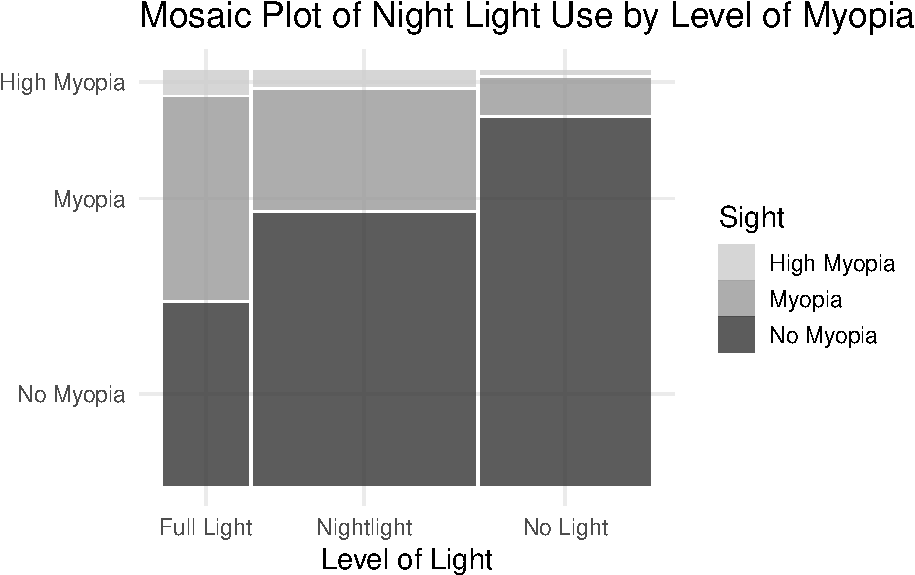
\includegraphics[width=0.6\linewidth]{08-A17-EDA-categorical_files/figure-latex/unnamed-chunk-4-1} \end{center}

\begin{enumerate}
\def\labelenumi{\arabic{enumi}.}
\setcounter{enumi}{11}
\tightlist
\item
  What is similar and what is different between the segmented bar chart and the mosaic bar chart?
\end{enumerate}

\vspace{1in}

\begin{enumerate}
\def\labelenumi{\arabic{enumi}.}
\setcounter{enumi}{12}
\tightlist
\item
  Explain why the bar for \texttt{Nightlight} is the widest in the mosaic plot.
\end{enumerate}

\vspace{0.8in}

\subsubsection*{Relative Risk}\label{relative-risk}
\addcontentsline{toc}{subsubsection}{Relative Risk}

\begin{enumerate}
\def\labelenumi{\arabic{enumi}.}
\setcounter{enumi}{13}
\tightlist
\item
  Calculate the relative risk of myopia for children that slept with full light compared to those that slept with no light.
\end{enumerate}

\vspace{0.8in}

\begin{enumerate}
\def\labelenumi{\arabic{enumi}.}
\setcounter{enumi}{14}
\tightlist
\item
  Interpret the value of relative risk in context of the problem.
\end{enumerate}

\vspace{1in}

\begin{enumerate}
\def\labelenumi{\arabic{enumi}.}
\setcounter{enumi}{15}
\tightlist
\item
  Calculate the percent increase/decrease in risk of myopia for children that slept with full light compared to those that slept with no light.
\end{enumerate}

\vspace{0.8in}

\begin{enumerate}
\def\labelenumi{\arabic{enumi}.}
\setcounter{enumi}{16}
\tightlist
\item
  Interpret as a percent increase/decrease in risk in context of the problem.
\end{enumerate}

\vspace{1in}

\subsection{Take-home messages}\label{take-home-messages-1}

\begin{enumerate}
\def\labelenumi{\arabic{enumi}.}
\item
  Bar charts can be used to graphically display a single categorical variable either as counts or proportions. Segmented bar charts and mosaic plots are used to display two categorical variables.
\item
  Segmented bar charts always have a scale from 0 - 100\%. The bars represent the outcomes of the explanatory variable. Each bar is segmented by the response variable. If the heights of each segment are the same for each bar there is no association between variables.
\item
  Mosaic plots are similar to segmented bar charts but the widths of the bars also show the number of observations within each outcome.
\end{enumerate}

\subsection{Additional notes}\label{additional-notes-1}

Use this space to summarize your thoughts and take additional notes on today's activity and material covered.

\newpage

\section{Activity 18: The Good Samaritan}\label{activity-18-the-good-samaritan}

\setstretch{1}

\subsection{Learning outcomes}\label{learning-outcomes-2}

\begin{itemize}
\item
  Given a research question involving two categorical variables, construct the null and alternative hypotheses
  in words and using appropriate statistical symbols.
\item
  Investigate the process of creating a null distribution for two categorical variables
\item
  Find and evaluate a p-value from the null distribution
\end{itemize}

\subsection{Terminology review}\label{terminology-review-2}

In today's activity, we will use simulation-based methods to analyze two categorical variables. Some terms covered in this activity are:

\begin{itemize}
\item
  Conditional proportion
\item
  Null hypothesis
\item
  Alternative hypothesis
\end{itemize}

To review these concepts, see Chapter 15 in your textbook.

\subsection{The Good Samaritan}\label{the-good-samaritan}

Researchers at the Princeton University wanted to investigate influences on behavior (Darley and Batson 1973). The researchers randomly selected 67 students from the Princeton Theological Seminary to participate in a study. Only 47 students chose to participate in the study, and the data below includes 40 of those students (7 students were removed from the study for various reasons). As all participants were theology majors planning a career as a preacher, the expectation was that all would have a similar disposition when it comes to helping behavior. Each student was then shown a 5-minute presentation on the Good Samaritan, a parable in the Bible which emphasizes the importance of helping others. After the presentation, the students were told they needed to give a talk on the Good Samaritan parable at a building across campus. Half the students were told they were late for the presentation; the other half told they could take their time getting across campus (the condition was randomly assigned). On the way between buildings, an actor pretending to be a homeless person in distress asked the student for help. The researchers recorded whether the student helped the actor or not. The results of the study are shown in the table below. Do these data provide evidence that those in a hurry will be less likely to help people in need in this situation? Use the order of subtraction hurry -- no hurry.

\begin{center}
\begin{tabular}{|c|c|c|c|}\hline
& Hurry Condition & No Hurry Condition & Total \\ \hline
Helped Actor & 2 & 11 & 13 \\ \hline
Did Not Help Actor & 18 & 9 & 27 \\ \hline
Total & 20 & 20 & 40 \\ \hline
\end{tabular}
\end{center}

These counts can be found in R by using the \texttt{count()} function:

\begin{itemize}
\item
  Download the R script file from D2L and upload to the RStudio server.
\item
  Highlight and run lines 1--7 to get the counts for each group.
\end{itemize}

\begin{Shaded}
\begin{Highlighting}[]
\CommentTok{\# Read data set in}
\NormalTok{good }\OtherTok{\textless{}{-}} \FunctionTok{read.csv}\NormalTok{(}\StringTok{"https://math.montana.edu/courses/s216/data/goodsam.csv"}\NormalTok{) }
\NormalTok{good }\SpecialCharTok{\%\textgreater{}\%} \FunctionTok{group\_by}\NormalTok{(Condition) }\SpecialCharTok{\%\textgreater{}\%} \FunctionTok{count}\NormalTok{(Behavior)}
\end{Highlighting}
\end{Shaded}

\begin{verbatim}
#> # A tibble: 4 x 3
#> # Groups:   Condition [2]
#>   Condition Behavior     n
#>   <chr>     <chr>    <int>
#> 1 Hurry     Help         2
#> 2 Hurry     No help     18
#> 3 No hurry  Help        11
#> 4 No hurry  No help      9
\end{verbatim}

\subsubsection*{Ask a research question}\label{ask-a-research-question}
\addcontentsline{toc}{subsubsection}{Ask a research question}

The research question as stated above is: Do these data provide evidence that those in a hurry will be less likely to help people in need in this situation? In order to set up our hypotheses, we need to express this research question in terms of parameters.

Remember, we define the parameter for a single categorical variable as the true proportion of observational units that are labeled as a ``success'' in the response variable.

For this study we are identifying two parameters and looking at the difference between these two parameters.

\begin{itemize}
\item
  \(\pi_\text{hurry}\) = long-run proportion of Princeton Theological Seminary students assigned to hurry that helped the actor
\item
  \(\pi_\text{no hurry}\) = long-run proportion of Princeton Theological Seminary students assigned not to hurry that helped the actor
\item
  \(\pi_\text{hurry} - \pi_\text{no hurry}\) = the difference in long-run proporiton of Princeton Theological Seminary Students that helped the actor between those who were assigned to hurry and those who were not assigned to hurry
\end{itemize}

When comparing two groups, we assume the two parameters are equal in the null hypothesis---there is no association between the variables.

\begin{enumerate}
\def\labelenumi{\arabic{enumi}.}
\tightlist
\item
  Write the null hypothesis out in words.
\end{enumerate}

\vspace{0.4in}

\begin{enumerate}
\def\labelenumi{\arabic{enumi}.}
\setcounter{enumi}{1}
\tightlist
\item
  Based on the research question, fill in the appropriate sign for the alternative hypothesis (\(<\), \(>\), or \(\neq\)):
  \vspace{2mm}
\end{enumerate}

~~~~~~~~~~\(H_A: \pi_{\text{hurry}} -\pi_{\text{no hurry}}\) \_\_\_\_\_\_\_\_\_\_ 0

\subsubsection*{Summarize and visualize the data}\label{summarize-and-visualize-the-data}
\addcontentsline{toc}{subsubsection}{Summarize and visualize the data}

To create the segmented bar plot:

\begin{itemize}
\item
  Enter the name of the explanatory variable for explanatory
\item
  Enter the name of the response variable for response
\item
  Highlight and run lines 13--20
\end{itemize}

\begin{Shaded}
\begin{Highlighting}[]
\NormalTok{good }\SpecialCharTok{\%\textgreater{}\%}
  \FunctionTok{ggplot}\NormalTok{(}\FunctionTok{aes}\NormalTok{(}\AttributeTok{x =}\NormalTok{ explanatory, }\AttributeTok{fill =}\NormalTok{ response))}\SpecialCharTok{+} \CommentTok{\#Enter the variables to plot}
  \FunctionTok{geom\_bar}\NormalTok{(}\AttributeTok{stat =} \StringTok{"count"}\NormalTok{, }\AttributeTok{position =} \StringTok{"fill"}\NormalTok{) }\SpecialCharTok{+}
  \FunctionTok{labs}\NormalTok{(}\AttributeTok{title =} \StringTok{"Segmented Bar Plot of Princeton Seminary Students that Help the actor }\SpecialCharTok{\textbackslash{}n}\StringTok{between those that were in a Hurry and those that were Not in a Hurry"}\NormalTok{,  }\CommentTok{\#Title your plot}
       \AttributeTok{y =} \StringTok{"Relative Frequency"}\NormalTok{, }\CommentTok{\#y{-}axis label}
       \AttributeTok{x =} \StringTok{"Condition"}\NormalTok{) }\SpecialCharTok{+} \CommentTok{\#x{-}axis label}
  \FunctionTok{scale\_fill\_grey}\NormalTok{()}
\end{Highlighting}
\end{Shaded}

\begin{enumerate}
\def\labelenumi{\arabic{enumi}.}
\setcounter{enumi}{2}
\tightlist
\item
  Based on the segmented bar plot, is there an association between whether a Seminary student helps the actor and condition assigned?
\end{enumerate}

\vspace{0.4in}

\begin{enumerate}
\def\labelenumi{\arabic{enumi}.}
\setcounter{enumi}{3}
\tightlist
\item
  Using the two-way table given in the introduction, calculate the conditional proportion of students in the hurry condition who helped the actor. Use appropriate notation.
\end{enumerate}

\vspace{.3in}

\begin{enumerate}
\def\labelenumi{\arabic{enumi}.}
\setcounter{enumi}{4}
\tightlist
\item
  Using the two-way table given in the introduction, calculate the conditional proportion of students in the no hurry condition who helped the actor. Use appropriate notation.
\end{enumerate}

\vspace{.3in}

\begin{enumerate}
\def\labelenumi{\arabic{enumi}.}
\setcounter{enumi}{5}
\tightlist
\item
  Calculate the summary statistic (difference in sample proportion) for this study. Use Hurry - No hurry as the order of subtraction. Use appropriate notation.
\end{enumerate}

\vspace{0.5in}

\textbf{Interpretation of the summary statistic:}

The proportion of Princeton Theological Seminary students that helped the actor is 0.45 less for those assigned to hurry compared to those assigned not to hurry.

\subsubsection*{Hypothesis Test}\label{hypothesis-test}
\addcontentsline{toc}{subsubsection}{Hypothesis Test}

We will now simulate a \textbf{null distribution} of sample differences in proportions. The null distribution is created under the assumption the null hypothesis is true.

\begin{enumerate}
\def\labelenumi{\arabic{enumi}.}
\setcounter{enumi}{6}
\tightlist
\item
  Using the cards provided by your instructor, simulate one sample under the assumption the null hypothesis is true.
\end{enumerate}

\begin{itemize}
\item
  Start with 40 cards (13 labeled helped, 27 labeled did not help)
\item
  Mix the cards together
\item
  Shuffle the cards into two piles (20 in hurry, 20 in no hurry)
\item
  Calculate the proportion of simulated students that helped in each group.
\item
  Report the difference in proportion of simulated students that helped (hurry - no hurry)
\end{itemize}

The segmented bar plot below shows the relationship between the variables for \textbf{one simulation assuming the null hypothesis is true}.

\begin{center}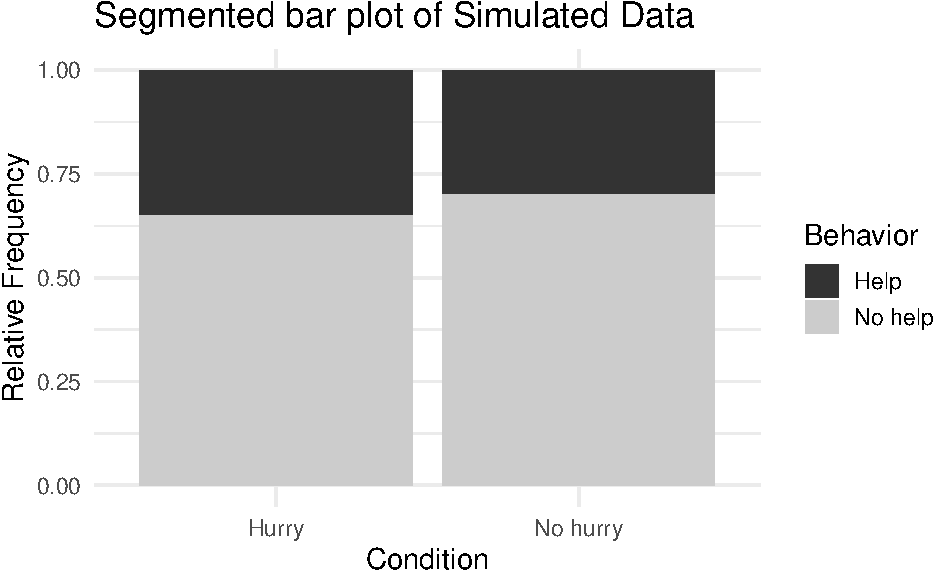
\includegraphics[width=0.6\linewidth]{08-A18-inference-2cat-simulationtest_files/figure-latex/unnamed-chunk-4-1} \end{center}

\newpage

To create the null distribution of differences in sample proportions, we will use the \texttt{two\_proportion\_test()} function in R (in the \texttt{catstats} package). We will need to enter the response variable name and the explanatory variable name for the formula, the data set name (identified above as \texttt{good}), the outcome for the explanatory variable that is first in subtraction, number of repetitions, the outcome for the response variable that is a success (what the numerator counts when calculating a sample proportion), and the direction of the alternative hypothesis.

The response variable name is \texttt{Behavior} and the explanatory variable name is \texttt{Condition}.

\begin{enumerate}
\def\labelenumi{\arabic{enumi}.}
\setcounter{enumi}{7}
\tightlist
\item
  What inputs should be entered for each of the following to create the simulation?
  \vspace{1mm}
\end{enumerate}

\begin{itemize}
\tightlist
\item
  First in subtraction (What is the outcome for the explanatory variable that is used as first in the order of subtraction? \texttt{"Hurry"} or \texttt{"No\ hurry"}):
\end{itemize}

\vspace{.15in}

\begin{itemize}
\tightlist
\item
  Number of repetitions:
\end{itemize}

\vspace{.15in}

\begin{itemize}
\tightlist
\item
  Response value numerator (What is the outcome for the response variable that is considered a success? \texttt{"Help"} or \texttt{"No\ help"}):
\end{itemize}

\vspace{.15in}

\begin{itemize}
\tightlist
\item
  As extreme as (enter the value for the sample difference in proportions):
\end{itemize}

\vspace{.15in}

\begin{itemize}
\tightlist
\item
  Direction (\texttt{"greater"}, \texttt{"less"}, or \texttt{"two-sided"}):
\end{itemize}

\vspace{.15in}

Using the R script file for this activity, enter your answers for question 8 in place of the \texttt{xx}'s to produce the null distribution with 1000 simulations; highlight and run lines 24--30.

\begin{Shaded}
\begin{Highlighting}[]
\FunctionTok{two\_proportion\_test}\NormalTok{(}\AttributeTok{formula =}\NormalTok{ Behavior}\SpecialCharTok{\textasciitilde{}}\NormalTok{Condition, }\CommentTok{\# response \textasciitilde{} explanatory}
    \AttributeTok{data =}\NormalTok{ good, }\CommentTok{\# Name of data set}
    \AttributeTok{first\_in\_subtraction =} \StringTok{"xx"}\NormalTok{, }\CommentTok{\# Order of subtraction: enter the name of Group 1}
    \AttributeTok{number\_repetitions =} \DecValTok{1000}\NormalTok{, }\CommentTok{\# Always use a minimum of 1000 repetitions}
    \AttributeTok{response\_value\_numerator =} \StringTok{"xx"}\NormalTok{, }\CommentTok{\# Define which outcome is a success}
    \AttributeTok{as\_extreme\_as =}\NormalTok{ xx, }\CommentTok{\# Calculated observed statistic (difference in sample proportions)}
    \AttributeTok{direction=}\StringTok{"xx"}\NormalTok{) }\CommentTok{\# Alternative hypothesis direction ("greater","less","two{-}sided")}
\end{Highlighting}
\end{Shaded}

\begin{enumerate}
\def\labelenumi{\arabic{enumi}.}
\setcounter{enumi}{8}
\tightlist
\item
  Sketch the null distribution created here.
\end{enumerate}

\vspace{1.5in}

\begin{enumerate}
\def\labelenumi{\arabic{enumi}.}
\setcounter{enumi}{9}
\tightlist
\item
  Explain why the null distribution is centered around the value of zero?
\end{enumerate}

\vspace{.8in}

\begin{enumerate}
\def\labelenumi{\arabic{enumi}.}
\setcounter{enumi}{10}
\tightlist
\item
  Interpret the p-value in context of the study.
\end{enumerate}

\vspace{1in}

\begin{enumerate}
\def\labelenumi{\arabic{enumi}.}
\setcounter{enumi}{11}
\tightlist
\item
  Write a conclusion in context of the study.
\end{enumerate}

\vspace{1in}

\subsection{Take-home messages}\label{take-home-messages-2}

\begin{enumerate}
\def\labelenumi{\arabic{enumi}.}
\tightlist
\item
  When comparing two groups, we are looking at the difference between two parameters. In the null hypothesis, we assume the two parameters are equal, or that there is no difference between the two proportions.
\end{enumerate}

\begin{enumerate}
\def\labelenumi{\arabic{enumi}.}
\setcounter{enumi}{1}
\tightlist
\item
  To create one simulated sample on the null distribution for a difference in sample proportions, label \(n_1 + n_2\) cards with the response variable outcomes from the original data. Mix cards together and shuffle into two new groups of sizes \(n_1\) and \(n_2\), representing the explanatory variable groups. Calculate and plot the difference in proportion of successes.
\end{enumerate}

\subsection{Additional notes}\label{additional-notes-2}

Use this space to summarize your thoughts and take additional notes on today's activity and material covered.

\newpage

\phantomsection\label{refs}
\begin{CSLReferences}{1}{0}
\bibitem[\citeproctext]{ref-pga}
{``Average Driving Distance and Fairway Accuracy.''} 2008. \href{https://www.pga.com/\%20and\%20https://www.lpga.com/}{https://www.pga.com/ and https://www.lpga.com/}.

\bibitem[\citeproctext]{ref-banton2022}
Banton, et al, S. 2022. {``Jog with Your Dog: Dog Owner Exercise Routines Predict Dog Exercise Routines and Perception of Ideal Body Weight.''} \emph{PLoS ONE} 17(8).

\bibitem[\citeproctext]{ref-bhavsar2022}
Bhavsar, et al, A. 2022. {``Increased Risk of Herpes Zoster in Adults \(\geq\)50 Years Old Diagnosed with COVID-19 in the United States.''} \emph{Open Forum Infectious Diseases} 9(5).

\bibitem[\citeproctext]{ref-islands}
Bulmer, M. n.d. {``Islands in Schools Project.''} \url{https://sites.google.com/site/islandsinschoolsprojectwebsite/home}.

\bibitem[\citeproctext]{ref-bts}
{``Bureau of Transportation Statistics.''} 2019. \url{https://www.bts.gov/}.

\bibitem[\citeproctext]{ref-babies}
{``Child Health and Development Studies.''} n.d. \url{https://www.chdstudies.org/}.

\bibitem[\citeproctext]{ref-darley1973}
Darley, J. M., and C. D. Batson. 1973. {``"From Jerusalem to Jericho": A Study of Situational and Dispositional Variables in Helping Behavior.''} \emph{Journal of Personality and Social Psychology} 27: 100--108.

\bibitem[\citeproctext]{ref-davis2020}
Davis, Smith, A. K. 2020. {``A Poor Substitute for the Real Thing: Captive-Reared Monarch Butterflies Are Weaker, Paler and Have Less Elongated Wings Than Wild Migrants.''} \emph{Biology Letters} 16.

\bibitem[\citeproctext]{ref-doit2015}
Du Toit, et al, G. 2015. {``Randomized Trial of Peanut Consumption in Infants at Risk for Peanut Allergy.''} \emph{New England Journal of Medicine} 372.

\bibitem[\citeproctext]{ref-edmunds2016}
Edmunds, et al, D. 2016. {``Chronic Wasting Disease Drives Population Decline of White-Tailed Deer.''} \emph{PLoS ONE} 11(8).

\bibitem[\citeproctext]{ref-ipeds}
Education Statistics, National Center for. 2018. {``IPEDS.''} \url{https://nces.ed.gov/ipeds/}.

\bibitem[\citeproctext]{ref-gbmarried}
{``Great Britain Married Couples: Great Britain Office of Population Census and Surveys.''} n.d. \url{https://discovery.nationalarchives.gov.uk/details/r/C13351}.

\bibitem[\citeproctext]{ref-zeitler2012}
Group, TODAY Study. 2012. {``\href{https://www.ncbi.nlm.nih.gov/pubmed/22540912}{A Clinical Trial to Maintain Glycemic Control in Youth with Type 2 Diabetes}.''} \emph{New England Journal of Medicine} 366: 2247--56.

\bibitem[\citeproctext]{ref-hamblin2007}
Hamblin, J. K., K. Wynn, and P. Bloom. 2007. {``Social Evaluation by Preverbal Infants.''} \emph{Nature} 450 (6288): 557--59.

\bibitem[\citeproctext]{ref-hirschfelder2018}
Hirschfelder, A., and P. F. Molin. 2018. {``I Is for Ignoble: Stereotyping Native Americans.''} \href{Retrieved\%20from\%20https://www.ferris.edu/HTMLS/news/jimcrow/native/homepage.htm.}{Retrieved from https://www.ferris.edu/HTMLS/news/jimcrow/native/homepage.htm.}

\bibitem[\citeproctext]{ref-hutchison2013}
Hutchison, R. L., and M. A. Hirthler. 2013. {``\href{https://www.ncbi.nlm.nih.gov/pubmed/23932117}{Upper Extremity Injuies in Homer's Iliad}.''} \emph{Journal of Hand Surgery (American Volume)} 38: 1790--93.

\bibitem[\citeproctext]{ref-imdb}
{``{IMDb} Movies Extensive Dataset.''} 2016. \url{https://kaggle.com/stefanoleone992/imdb-extensive-dataset}.

\bibitem[\citeproctext]{ref-kalra2022}
Kalra, et al., Dl. 2022. {``Trustworthiness of Indian Youtubers.''} Kaggle. \url{https://doi.org/10.34740/KAGGLE/DSV/4426566}.

\bibitem[\citeproctext]{ref-keating2021}
Keating, D., N. Ahmed, F. Nirappil, Stanley-Becker I., and L. Bernstein. 2021. {``Coronavirus Infections Dropping Where People Are Vaccinated, Rising Where They Are Not, Post Analysis Finds.''} \emph{Washington Post}. \url{https://www.washingtonpost.com/health/2021/06/14/covid-cases-vaccination-rates/}.

\bibitem[\citeproctext]{ref-laeng2007}
Laeng, Mathisen, B. 2007. {``Why Do Blue-Eyed Men Prefer Women with the Same Eye Color?''} \emph{Behavioral Ecology and Sociobiology} 61(3).

\bibitem[\citeproctext]{ref-levin2000}
Levin, D. T. 2000. {``Race as a Visual Feature: Using Visual Search and Perceptual Discrimination Tasks to Understand Face Categories and the Cross-Race Recognition Deficit.''} \emph{Journal of Experimental Psychology} 129(4).

\bibitem[\citeproctext]{ref-luetkemeier2017}
LUETKEMEIER, et al., M. 2017. {``Skin Tattoos Alter Sweat Rate and Na+ Concentration.''} \emph{Medicine and Science in Sports and Exercise} 49(7).

\bibitem[\citeproctext]{ref-madden2020}
Madden, et al, J. 2020. {``Ready Student One: Exploring the Predictors of Student Learning in Virtual Reality.''} \emph{PLoS ONE} 15(3).

\bibitem[\citeproctext]{ref-miller1956}
Miller, G. A. 1956. {``The Magical Number Seven, Plus or Minus Two: Some Limits on Our Capacity for Processing Information.''} \emph{Psychological Review} 63(2).

\bibitem[\citeproctext]{ref-becentispeech}
Moquin, W., and C. Van Doren. 1973. {``Great Documents in American Indian History.''} Praeger.

\bibitem[\citeproctext]{ref-pew2022}
{``More Americans Are Joining the 'Cashless' Economy.''} 2022. \url{https://www.pewresearch.org/short-reads/2022/10/05/more-americans-are-joining-the-cashless-economy/.}

\bibitem[\citeproctext]{ref-weather}
National Weather Service Corporate Image Web Team. n.d. {``National Weather Service -- {NWS} Billings.''} \url{https://w2.weather.gov/climate/xmacis.php?wfo=byz}.

\bibitem[\citeproctext]{ref-obrien2019}
O'Brien, Lynch, H. D. 2019. {``Crocodylian Head Width Allometry and Phylogenetic Prediction of Body Size in Extinct Crocodyliforms.''} \emph{Integrative Organismal Biology} 1.

\bibitem[\citeproctext]{ref-ocean}
{``Ocean Temperature and Salinity Study.''} n.d. \url{https://calcofi.org/}.

\bibitem[\citeproctext]{ref-WashPost2022}
{``Older People Who Get Covid Are at Increased Risk of Getting Shingles.''} 2022. \url{https://www.washingtonpost.com/health/2022/04/19/shingles-and-covid-over-50/.}

\bibitem[\citeproctext]{ref-physhealth}
{``Physician's Health Study.''} n.d. \url{https://phs.bwh.harvard.edu/}.

\bibitem[\citeproctext]{ref-porath2017}
Porath, Erez, C. 2017. {``Does Rudeness Really Matter? The Effects of Rudeness on Task Performance and Helpfulness.''} \emph{Academy of Management Journal} 50.

\bibitem[\citeproctext]{ref-quinn1999}
Quinn, G. E., C. H. Shin, M. G. Maguire, and R. A. Stone. 1999. {``Myopia and Ambient Lighting at Night.''} \emph{Nature} 399 (6732): 113--14. \url{https://doi.org/10.1038/20094}.

\bibitem[\citeproctext]{ref-ramachandran2007}
Ramachandran, V. 2007. {``3 Clues to Understanding Your Brain.''} \url{https://www.ted.com/talks/vs_ramachandran_3_clues_to_understanding_your_brain}.

\bibitem[\citeproctext]{ref-cdchospitalization}
{``Rates of Laboratory-Confimed COVID-19 Hospitalizations by Vaccination Status.''} 2021. CDC. \url{https://covid.cdc.gov/covid-data-tracker/\#covidnet-hospitalizations-vaccination}.

\bibitem[\citeproctext]{ref-richardson2019}
Richardson, T., and R. T. Gilman. 2019. {``Left-Handedness Is Associated with Greater Fighting Success in Humans.''} \emph{Scientific Reports} 9 (1): 15402. \url{https://doi.org/10.1038/s41598-019-51975-3}.

\bibitem[\citeproctext]{ref-stephens2020}
Stephens, R., and O. Robertson. 2020. {``Swearing as a Response to Pain: Assessing Hypoalgesic Effects of Novel "Swear" Words.''} \emph{Frontiers in Psychology} 11: 643--62.

\bibitem[\citeproctext]{ref-stewart2014}
Stewart, E. H., B. Davis, B. L. Clemans-Taylor, B. Littenberg, C. A. Estrada, and R. M. Centor. 2014. {``Rapid Antigen Group a Streptococcus Test to Diagnose Pharyngitis: A Systematic Review and Meta-Analysis''} 9 (11). \url{https://doi.org/10.1371/journal.pone.0111727}.

\bibitem[\citeproctext]{ref-stroop1935}
Stroop, J. R. 1935. {``Studies of Interference in Serial Verbal Reactions.''} \emph{Journal of Experimental Psychology} 18: 643--62.

\bibitem[\citeproctext]{ref-subach2022}
Subach, et al, A. 2022. {``Foraging Behaviour, Habitat Use and Population Size of the Desert Horned Viper in the Negev Desert.''} \emph{Soc.Open Sci} 9.

\bibitem[\citeproctext]{ref-sulheim2017}
Sulheim, S., A. Ekeland, I. Holme, and R. Bahr. 2017. {``Helmet Use and Risk of Head Injuries in Alpine Skiers and Snowboarders: Changes After an Interval of One Decade''} 51 (1): 44--50. \url{https://doi.org/10.1136/bjsports-2015-095798}.

\bibitem[\citeproctext]{ref-titanic}
{``Titanic.''} n.d. \url{http://www.encyclopedia-titanica.org}.

\bibitem[\citeproctext]{ref-covidvaccinetracker}
{``US COVID-19 Vaccine Tracker: See Your State's Progress.''} 2021. Mayo Clinic. \url{https://www.mayoclinic.org/coronavirus-covid-19/vaccine-tracker}.

\bibitem[\citeproctext]{ref-usepa2020}
US Environmental Protection Agency. n.d. {``Air Data -- Daily Air Quality Tracker.''} \url{https://www.epa.gov/outdoor-air-quality-data/air-data-daily-air-quality-tracker}.

\bibitem[\citeproctext]{ref-wahlstrom2014}
Wahlstrom, et al, K. 2014. {``Examining the Impact of Later School Start Times on the Health and Academic Performance of High School Students: A Multi-Site Study.''} \emph{Center for Applied Research and Educational Improvement}.

\bibitem[\citeproctext]{ref-watson2015}
Watson, et al., N. 2015. {``Recommended Amount of Sleep for a Heathy Adult: A Joint Consensus Statement of the American Academy of Sleep Medicine and Sleep Research Society.''} \emph{Sleep} 38(6).

\bibitem[\citeproctext]{ref-Weiss1988}
Weiss, R. D. 1988. {``Relapse to Cocaine Abuse After Initiating Desipramine Treatment.''} \emph{JAMA} 260(17).

\bibitem[\citeproctext]{ref-navajo2011}
{``Welcome to the Navajo Nation Government: Official Site of the Navajo Nation.''} 2011.\href{\%20Retrieved\%20from\%20https://www.navajo-nsn.gov/.}{Retrieved from https://www.navajo-nsn.gov/.}

\bibitem[\citeproctext]{ref-wilson2016}
Wilson, Woodruff, J. P. 2016. {``Vertebral Adaptations to Large Body Size in Theropod Dinosaurs.''} \emph{PLoS ONE} 11(7).

\end{CSLReferences}

\end{document}
